\mode*
\section{From Power Up To Bash Prompt}

\subsection{Motherboard Chipsets And The Memory Map}

Ref: \citetitle{duarte:gustavo2008chipsets}

\begin{frame}\mode<beamer>{\frametitle{Motherboard Chipsets And The Memory Map}}
  \begin{center}
    \mode<beamer>{ 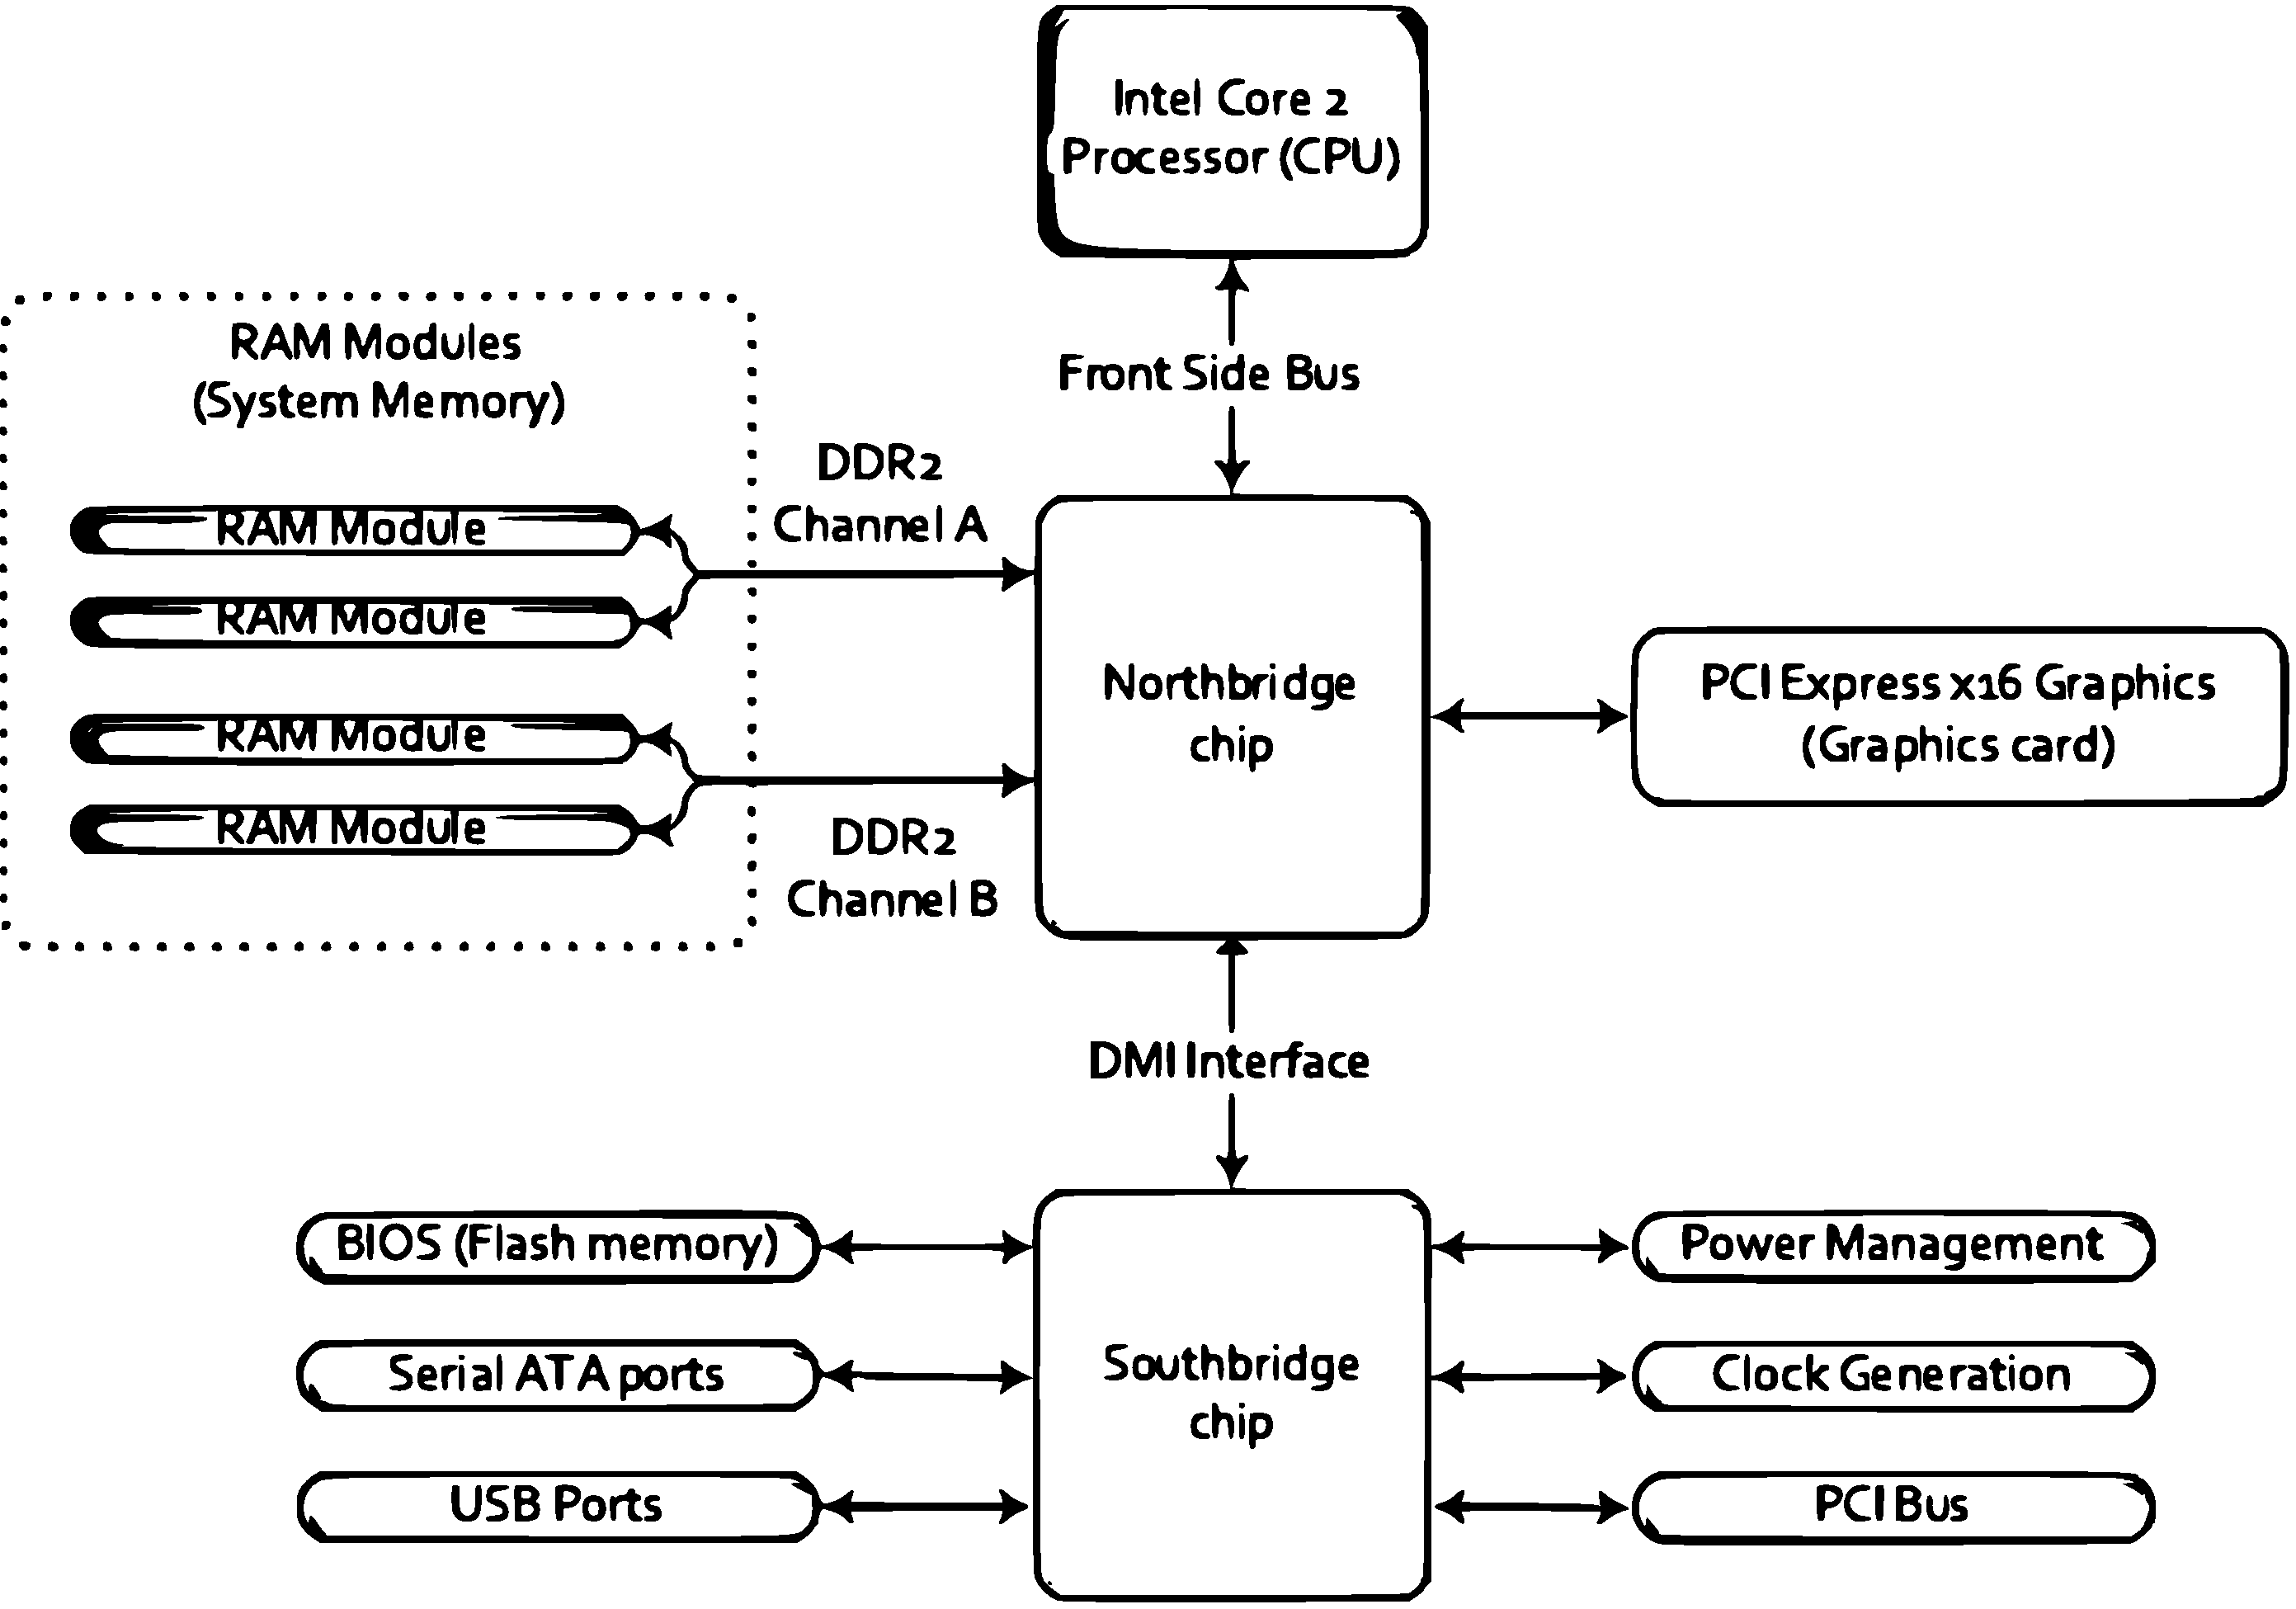
\includegraphics[width=\textwidth]{motherboardDiagram} }
    \mode<article>{ 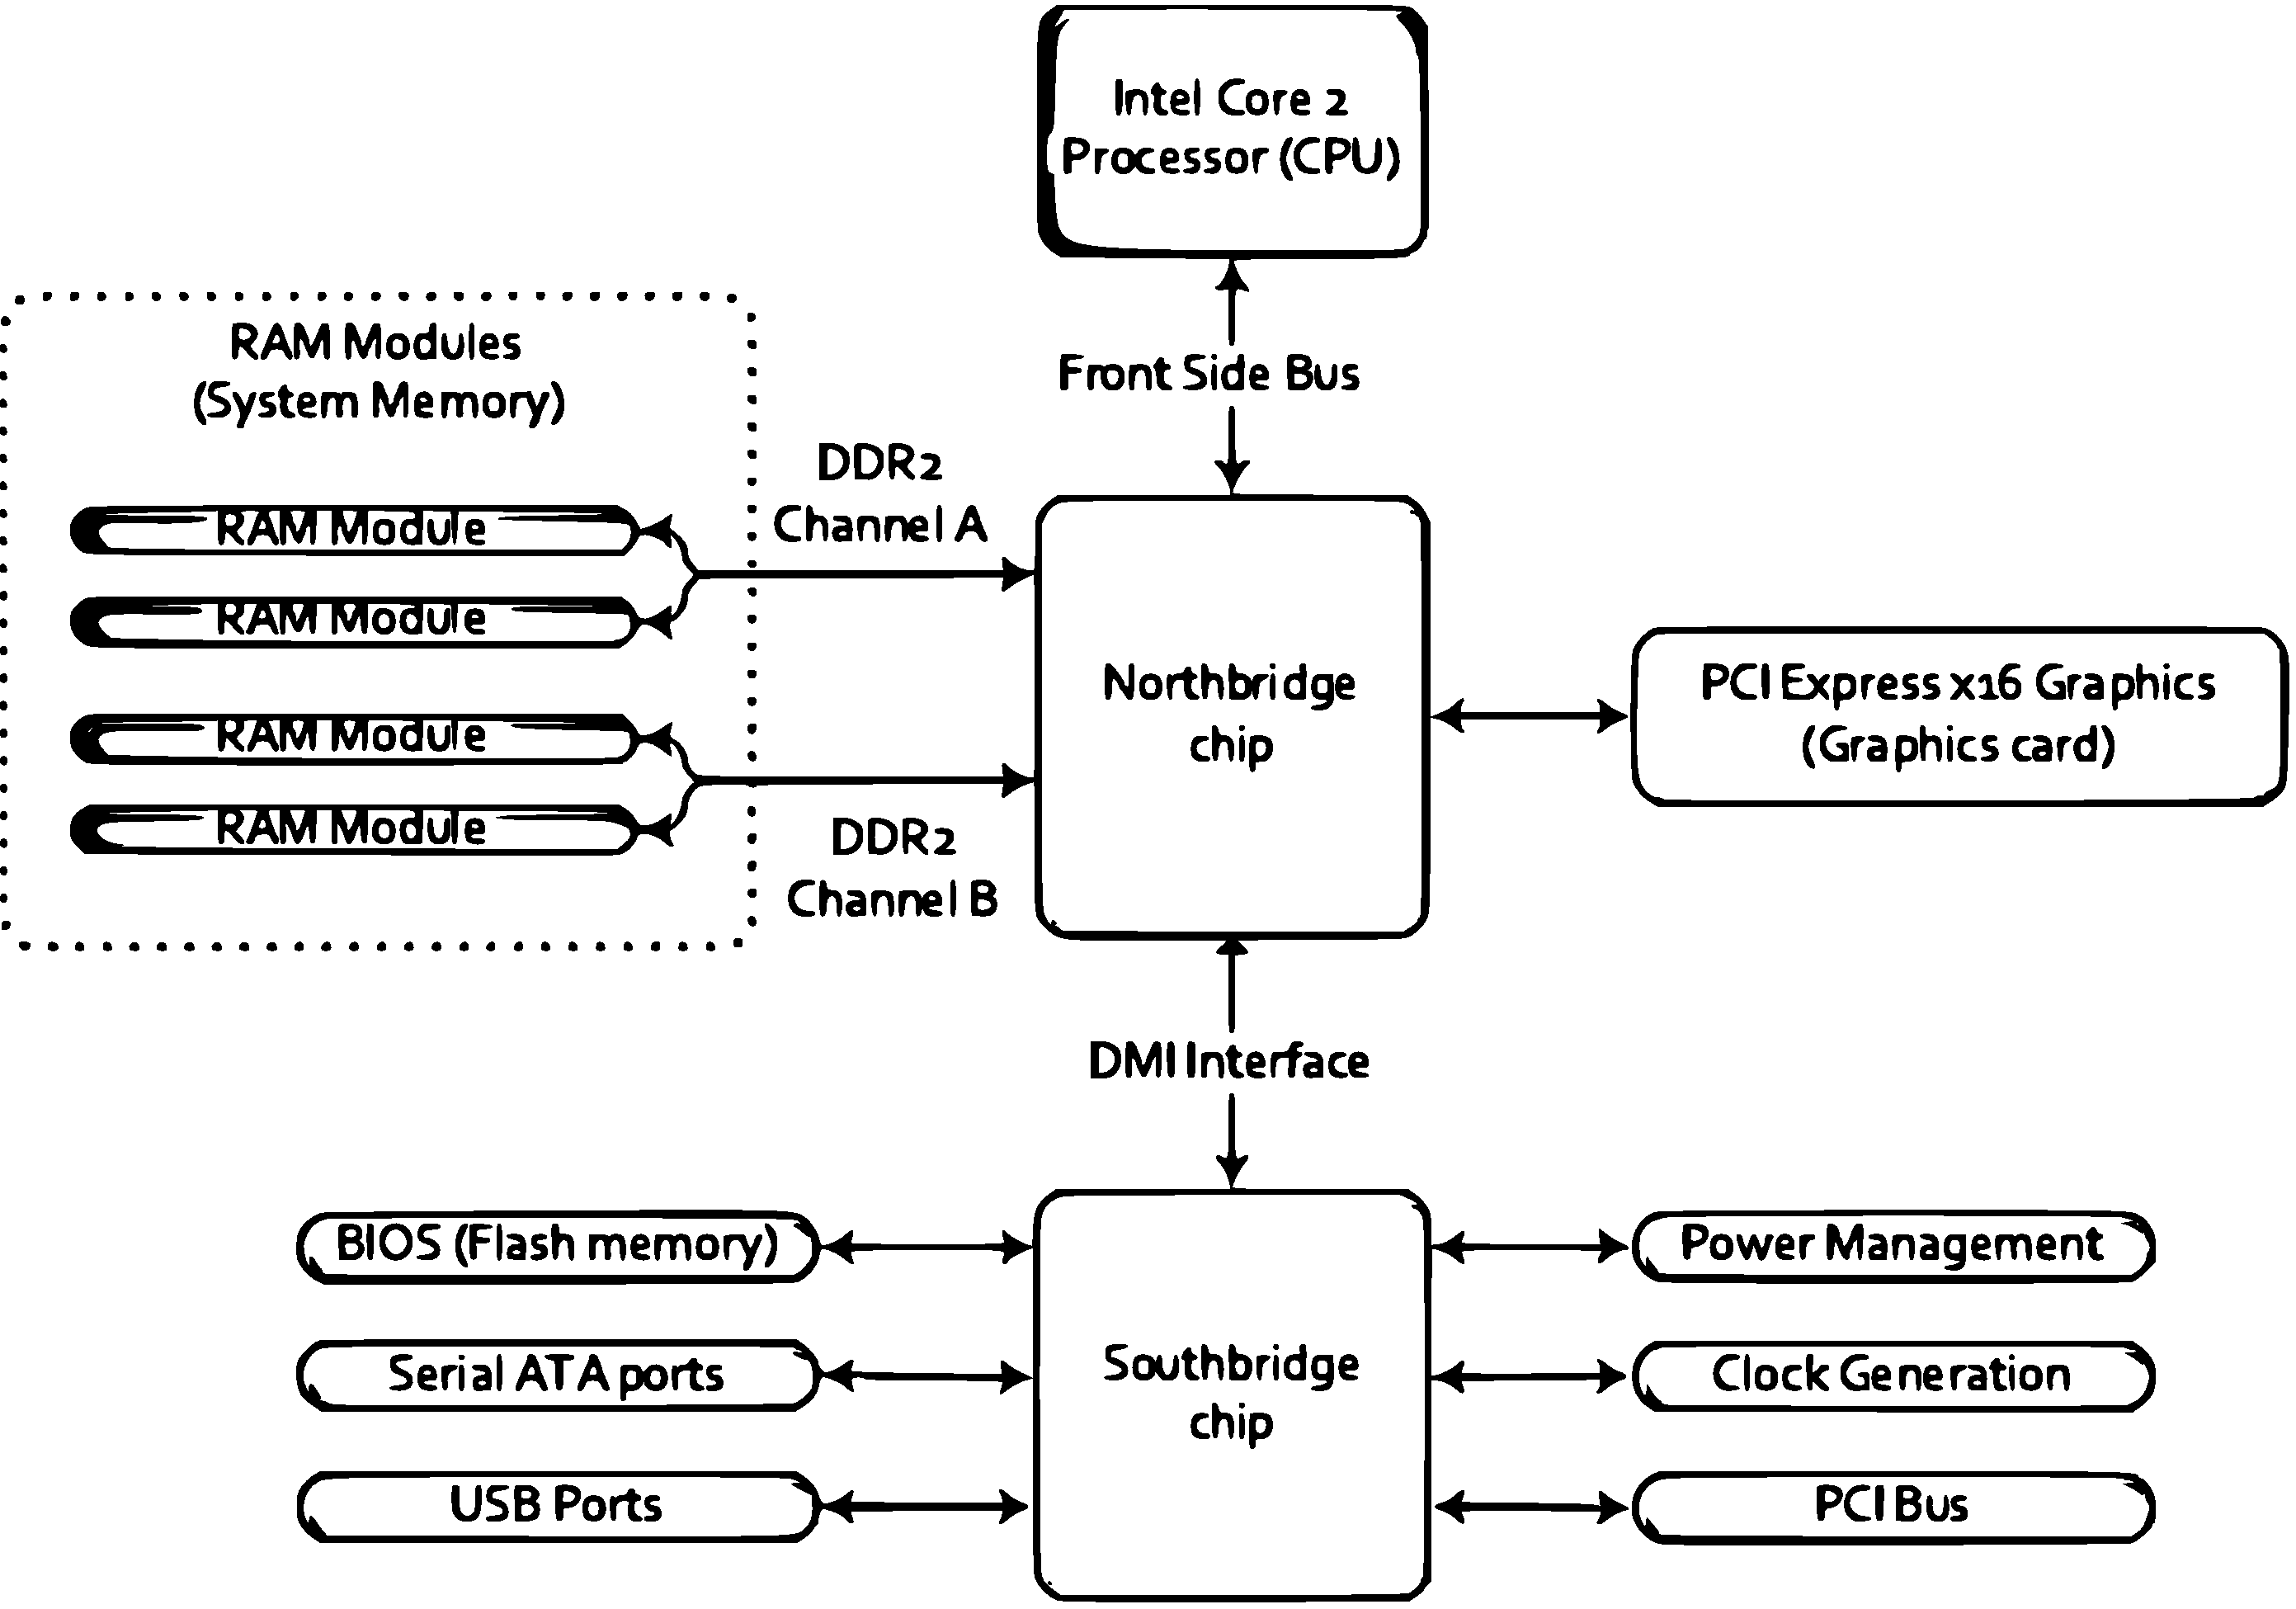
\includegraphics[width=.6\textwidth]{motherboardDiagram} }
  \end{center}
\end{frame}

\begin{frame}
  \begin{block}{Facts}
    \begin{itemize}
    \item The CPU doesn't know what it's connected to
      \begin{itemize}
      \item[-] CPU test bench?\quad{}network router?\quad{}toaster?\quad{}brain implant?
      \end{itemize}
    \item The CPU talks to the outside world through its pins
      \begin{itemize}
      \item[-] some pins to transmit the physical memory address
      \item[-] other pins to transmit the values
      \end{itemize}
    \item The CPU's gateway to the world is the front-side bus
    \end{itemize}
  \end{block}
  \begin{block}{Intel Core 2 QX6600}
    \begin{itemize}
    \item 33 pins to transmit the physical memory address
      \begin{itemize}
      \item[-] so there are $2^{33}$ choices of memory locations
      \end{itemize}
    \item 64 pins to send or receive data
      \begin{itemize}
      \item[-] so data path is 64-bit wide, or 8-byte chunks
      \end{itemize}
    \end{itemize}
    This allows the CPU to physically address 64GB of memory ($2^{33}\times{}8B$)
  \end{block}
\end{frame}

See also: \href{http://download.intel.com/design/processor/datashts/31559205.pdf}{\emph{Datasheet for Intel Core 2 Quad-Core Q6000
  Sequence}}\footnote{\url{http://download.intel.com/design/processor/datashts/31559205.pdf}}

\begin{frame}%{Motherboard Chipsets And The Memory Map}{ --- Facts}
  \begin{minipage}{.59\textwidth}
    \textcolor{blue}{Some physical memory addresses are mapped away!}
    \begin{itemize}
    \item only the addresses, not the spaces
    \item Memory holes
      \begin{itemize}
      \item[-] $640KB \sim 1MB$
      \item[-] /proc/iomem
      \end{itemize}
    \item Memory-mapped I/O
      \begin{itemize}
      \item BIOS ROM
      \item video cards
      \item PCI cards
      \item ...
      \end{itemize}
    \end{itemize}
    This is why 32-bit OSes have problems using 4G of RAM.
  \end{minipage}\hfill
  \begin{minipage}{.39\textwidth}
    \begin{center}
      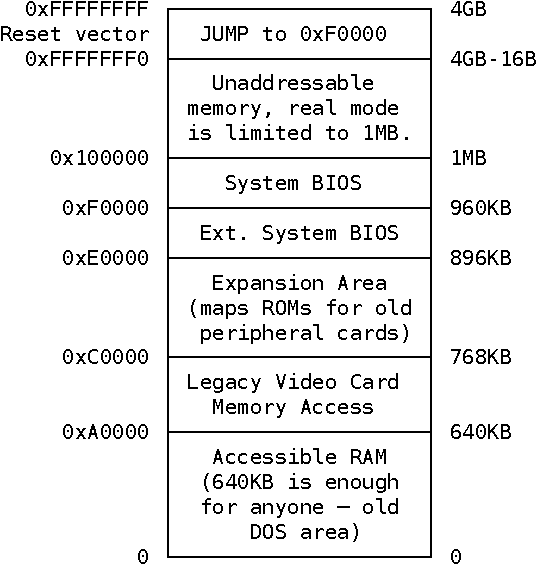
\includegraphics[width=1.2\textwidth]{boot-mem}
    \end{center}
  \end{minipage}
  \vspace{1em}
  \begin{center}
    What if you don't have 4G RAM?
  \end{center}
\end{frame}

See also: \href{http://wiki.osdev.org/Memory_Map_(x86)}{\emph{Memory Map (x86)}}\footnote{\url{http://wiki.osdev.org/Memory_Map_(x86)}}

\begin{frame}%{Motherboard Chipsets And The Memory Map}{ --- Facts}
  \begin{block}{the northbridge}
    \begin{enumerate}
    \item receives a physical memory request
    \item decides where to route it
      \begin{itemize}
      \item[-] to RAM? to video card? to ...?
      \item[-] decision made via the \emph{memory address map}
        \begin{itemize}
        \item \texttt{/proc/iomem}
        \item it is built in \texttt{setup()}
        \end{itemize}
      \end{itemize}
    \end{enumerate}
  \end{block}
\end{frame}

% \begin{itemize}
% \item When is the memory address map built? \code{setup()}.
% \end{itemize}

\begin{frame}%{Motherboard Chipsets And The Memory Map}{ --- Facts}
  \begin{block}{The CPU modes}
    \begin{description}
    \item[real mode:] CPU can only address 1MB RAM
      \begin{itemize}
      \item 20-bit address, 1-byte data unit
      \end{itemize}
    \item[32-bit protected mode:] can address 4GB RAM
      \begin{itemize}
      \item 32-bit address, 1-byte data unit
      \end{itemize}
    \item[64-bit protected mode:] can address 64GB RAM (Intel Core 2 QX6600)
      \begin{itemize}
      \item 33 address pins, 8-byte data unit
      \end{itemize}
    \end{description}
  \end{block}
  \begin{itemize}
  \item[\$] \texttt{grep 'address sizes' /proc/cpuinfo}
  \end{itemize}
\end{frame}

The \emph{physical} stuff is determined by hard-core limits: the actual metal pins that
stick out of the processor. It is \emph{those} pins that limit the CPU to 64
gigabytes. That is completely independent of the operating system or even the mode
(real-mode, 32-bit protected, 64-bit) the CPU is running in. It's a physical limit. That
is the limit for which that little multiplication is done. There are 33 metal pins to
transmit an address and 8 metal pins to send and receive data. So
$2^{33}\times{} 2^3 = 2^{36} = 64 GB$.  The “unit” of transfer in this case is 8 bytes,
that's the smallest chunk of data the CPU can address on the physical bus. In actuality,
the CPU usually works in terms of cache lines, which hold 64 bytes in the Core 2s. Due to
performance, the CPU reads a whole cache line at a time. So if a program reads one byte,
the CPU actually reads 64 bytes and stores them in the cache.  The 4-gb limit is logical,
not physical. It happens because the registers and instructions in the CPU are limited to
32 bits \emph{when it's running in 32-bit mode}, which \emph{does} depend on the
OS. Programs need to be able to address individual bytes in memory, so the “unit” of
addressing is 1 byte. So \emph{that} equation becomes
$2^{32}\ addresses \times{} 1\ byte\ chunks = 2^{32}\ bytes$, or 4 GB total
addressing. (The comments in \citetitle{duarte:gustavo2008chipsets})

\subsection{How Computers Boot Up}

Ref: \citetitle{duarte:gustavo2008boot}

\begin{frame}{Bootstrapping}
  \begin{center}
    \mode<beamer>{ 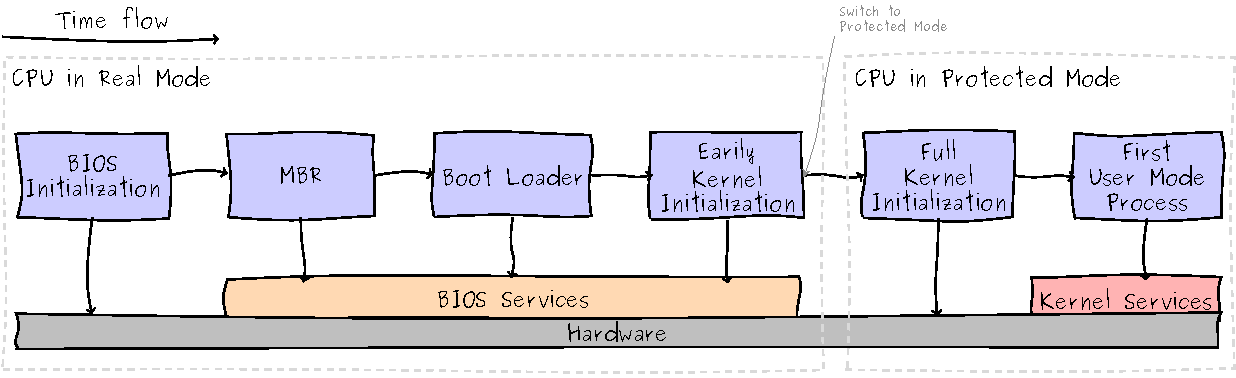
\includegraphics[width=\textwidth]{boot} }
    \mode<article>{ \includegraphics[width=.8\textwidth]{boot-bw} }
  \end{center}
  \begin{enumerate}
  \item bringing at least a portion of the OS into main memory, and
  \item having the processor execute it
  \item the initialization of kernel data structures
  \item the creation of some user processes, and
  \item the transfer of control to one of them
  \item[\$] \texttt{man 7 boot}
  \end{enumerate}
\end{frame}

\subsubsection{Motherboard power up}

\begin{frame}
  \begin{block}{Motherboard power up}
    \begin{enumerate}
    \item initializes motherboard firmwares (chipset, etc.)
    \item gets CPU running
    \end{enumerate}
  \end{block}
\end{frame}

\begin{frame}{Real mode}{CPU acts as a 1978 Intel 8086}
  \begin{minipage}{.52\textwidth}
    \begin{itemize}
    \item any code can write to any place in memory
    \item only 1MB of memory can be addressed
    \item registers are initialized
      \begin{itemize}
      \item[-] \texttt{EIP} has \texttt{0xFFFFFFF0}, the \textcolor{blue}{reset vector}
      \item[-] at the reset vector, there is a \texttt{jump} instruction, jumping to the
        \emph{BIOS entry point} (\texttt{0xF0000}).%\ (960KB), 64KB below 1MB)
      \end{itemize}
    \end{itemize}
  \end{minipage}\hfill
  \begin{minipage}{.48\textwidth}
    \begin{center}
      \mode<beamer>{ 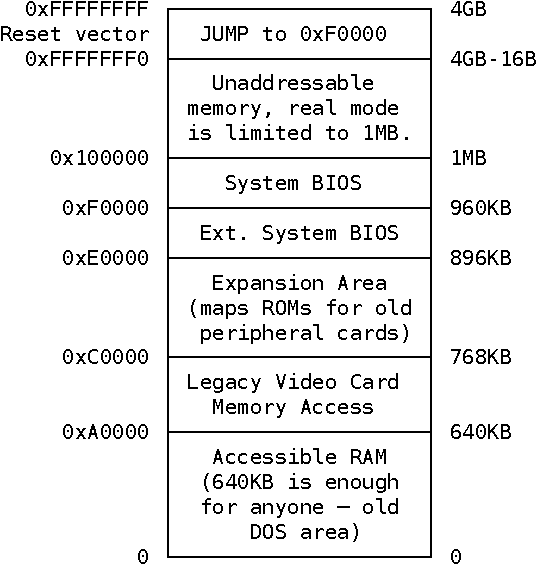
\includegraphics[width=1.15\textwidth]{boot-mem} }
      \mode<article>{ 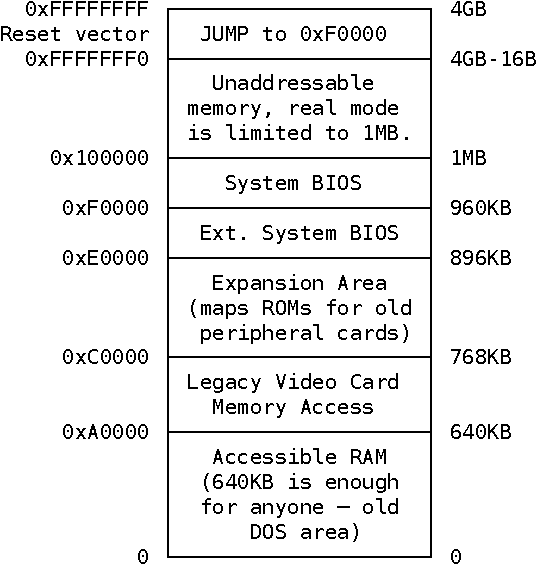
\includegraphics[width=.7\textwidth]{boot-mem} }
    \end{center}
  \end{minipage}
\end{frame}

See also:
\begin{itemize}
\item \citetitle{web:bios-rom}
\item \citetitle{web:boot-seq}
\item \citetitle{web:bios-rom2}
\item \citetitle{wiki:rst-vector}
\item \citetitle{web:boot-cpu}
\end{itemize}

\subsubsection{BIOS}

\begin{frame}\mode<beamer>{\frametitle{BIOS}}
  \begin{block}{BIOS uses Real Mode addresses}
    \begin{itemize}
    \item No GDT, LDT, or paging table is needed
      \begin{itemize}
      \item the code that initializes the GDT, LDT, and paging tables must run in Real Mode
      \end{itemize}
    \item Real mode address translation:
      $$\mathtt{segment number}\times{}2^4+\mathtt{offset}$$
      \begin{itemize}
      \item[e.g.] to translate \texttt{<FFFF:0001>} into physical address:
        $$FFFF \times{} 16 + 0001 = FFFF0 + 0001 = FFFF1$$
      \item[if:] \texttt{offset > 0xF} (overflow)
      \item[then:] $\mathtt{address \% 2^{20}}$ (wrap around)
      \item only 80286 and later x86 CPUs can address up to:
        $$FFFF0 + FFFF = 10FFEF$$
      \end{itemize}
    \end{itemize}
  \end{block}
\end{frame}

See also:
\begin{itemize}
\item \citetitle[Sec.~1.3, \emph{The BIOS}]{freebsd:archbook}
\item \citetitle{wiki:realmode}
\item \citetitle{osdev:realmode} 
\end{itemize}

\begin{frame}{CPU starts executing BIOS code}
  \begin{enumerate}
  \item POST
    \begin{itemize}
    \item an ACPI-compliant BIOS builds several tables that describe the hardware devices
      present in the system
    \end{itemize}
  \item initializes hardwares
    \begin{itemize}
    \item at the end of this phase, a table of installed PCI devices is displayed
    \end{itemize}
  \item find a boot device
  \item load MBR into \texttt{0x7c00}
  \item Jump to \texttt{0x7c00}
  \item MBR moves itself away from \texttt{0x7c00}% (fig~\ref{fig:boot-mem3})
  \end{enumerate}
  \begin{center}
    \mode<beamer>{
      \includegraphics[width=\textwidth]{mbr}
    } \mode<article>{
      \includegraphics[width=.6\textwidth]{mbr}
    }
  \end{center}
\end{frame}

\begin{minipage}{.65\textwidth}
  \begin{itemize}
  \item The MBR includes a small boot loader, which is loaded into RAM starting from
    address \texttt{0x00007c00} by the BIOS.

    \begin{itemize}
    \item \href{http://www.glamenv-septzen.net/en/view/6}{Why \texttt{0x7c00}?}\footnote{\url{http://www.glamenv-septzen.net/en/view/6}}
    \end{itemize}

  \item This small program
    \begin{enumerate}
    \item moves itself to the address \texttt{0x00096a00},
      \begin{itemize}
      \item Why? because the boot loader may copy the boot sector of a boot
        partition into RAM (\texttt{0x7c00}) and execute it
      \end{itemize}
    \item sets up the real mode stack (ranging from \texttt{0x00098000} to
      \texttt{0x000969ff}),
    \item loads the second part of the boot loader into RAM starting from address
      \texttt{0x00096c00}, and jumps into it.
    \end{enumerate}
  \end{itemize}
\end{minipage}\hfill
\begin{minipage}{.3\textwidth}
  \includegraphics[width=\textwidth]{boot-mem3}
\end{minipage}

\subsubsection{The Boot Loader}

\begin{frame}[fragile=singleslide]{GRUB}
  \begin{enumerate}
  \item GRUB stage 1 (in MBR) loads GRUB stage 2
  \item stage 2 reads GRUB configuration file, and presents boot menu
  \item loads the kernel image file into memory% (fig~\ref{fig:boot-mem3})
    \begin{itemize}
    \item can't be done in real mode, since it's bigger than 640KB
      \begin{itemize}
      \item BIOS supports \emph{unreal mode}
      \end{itemize}
    \item 1\textsuperscript{st} 512 bytes --- \texttt{INITSEG, 0x00090000}
    \item \texttt{setup()} --- \texttt{SETUPSEG, 0x00090200}
    \item load low --- \texttt{SYSSEG, 0x00010000}
    \item load high --- \texttt{0x00100000}
    \end{itemize}
  \item jumps to the kernel entry point (\mintinline{gas}{jmp trampoline})
    \begin{itemize}
    \item line 80 in \texttt{2.6.11/arch/i386/boot/setup.S}
    \end{itemize}
  \end{enumerate}
\end{frame}

``\mintinline{gas}{jmp trampoline}'' was used in 2.6.11 for calling \texttt{start\_of\_setup}. In
newer kernels, a \emph{2-byte jump} is used instead.

See also:
\begin{itemize}
\item \href{http://www.dedoimedo.com/computers/grub.html}{\emph{GRUB bootloader - Full
      tutorial}}\footnote{\url{http://www.dedoimedo.com/computers/grub.html}}
\item Kernel source v2.6.34:
  \href{http://lxr.linux.no/linux+v2.6.34/arch/x86/boot/header.S\#L112}{\emph{\texttt{header.S}}}\footnote{\url{http://lxr.linux.no/linux+v2.6.34/arch/x86/boot/header.S\#L112}}
\item \href{http://thestarman.pcministry.com/asm/2bytejumps.htm}{\emph{Using SHORT
      (Two-byte) Relative Jump
      Instructions}}\footnote{\url{http://thestarman.pcministry.com/asm/2bytejumps.htm}}
\item \href{http://www.groad.net/bbs/read.php?tid-3001.html}{\emph{2-byte jump in
      \texttt{header.S}}}\footnote{\url{http://www.groad.net/bbs/read.php?tid-3001.html}}
\end{itemize}

\paragraph{More about unreal mode}

Unreal Mode is a ``mode'' where the processor runs in real mode while the segment limit
does not equal 64KB (in most cases, its 4GB). Since real mode doesn't update the limit
field (of the cache), this state persists across segment register loads. Entering this
mode is achieved easily by entering protected mode (where the limit can be changed), load
the desired limit into the descriptor cache, then switch back to real
mode. \citetitle{osdev:descriptor-cache}

The benefits of unreal mode are quite well known: access to the 32-bit address space while
simultaneously being able to call BIOS and real mode programs. \citetitle{osdev:unrealmode2}

See also:
\begin{itemize}
\item \href{http://forum.osdev.org/viewtopic.php?f=1\&t=21179\&start=15}{A great post in OSDev forum: \emph{Unreal
  mode}}\footnote{\url{http://forum.osdev.org/viewtopic.php?f=1&t=21179&start=15}} that
deserves a detailed look.
\item OSDev:
  \href{http://files.osdev.org/mirrors/geezer/johnfine/segments.htm}{\emph{Segment
      Registers: Real mode vs. Protected mode}} covers \emph{unreal mode}, \emph{NULL
    selector}, \emph{mode
    switching}\footnote{\url{http://files.osdev.org/mirrors/geezer/johnfine/segments.htm}}.
\item \citetitle{osdev:realmode2}
\item \citetitle{wiki:unrealmode}
\item \citetitle{osdev:unrealmode}
\end{itemize}

\begin{figure}[h]
  \centering
  \includegraphics[width=.4\textwidth]{nonprogrammable}
  \caption{Descriptor cache register}
  \label{fig:cache-register}
\end{figure}

\paragraph{More about \emph{bootloader}:}
\begin{enumerate}
\item display a ``Loading'' message
\item load an initial portion of the kernel image from disk:
  \begin{enumerate}
  \item the first 512 bytes of the kernel image are put in RAM at address
    \texttt{0x00090000} (576K, \texttt{INITSEG})
    \begin{itemize}
    \item \mintinline{sh}{hd -n512 /boot/vmlinuz-3.2.0-1-amd64}
    \item \texttt{/usr/src/linux/arch/i386/boot/bootsect.S}
    \item it was a floppy boot loader, and no longer valid since 2.6
    \item nowadays to make a bootable floppy, you have to use a bootloader as you do with
      a hard disk
    \end{itemize}
  \item the code of the \texttt{setup()} function (see below) is put in RAM starting
    from address \texttt{0x00090200} ($576K+512$, \texttt{SETUPSEG})
  \end{enumerate}
\item load the rest of the kernel image from disk and puts the image in RAM starting from
  either low address \texttt{0x00010000} (64K, \texttt{SYSSEG}) (for small kernel images
  ($< 512K$) compiled with ``\mintinline{sh}{make zImage}'') or high address
  \texttt{0x00100000} (1M)(for big kernel images ($> 512K$) compiled with \mintinline{sh}{make
    bzImage}).
  \begin{description}
  \item[ISA hole:] Physical addresses ranging from \texttt{0x000a0000} (640K) to
    \texttt{0x000fffff} ($1M-1$) are usually reserved to BIOS routines and to map the
    internal memory of ISA graphics cards
  \end{description}
\item Jumps to the \texttt{setup()} code. (\texttt{/usr/src/linux/arch/i386/boot/setup.S})
\end{enumerate}

\begin{description}
\item[BIOS interrupt call] \mintinline{gas}{int $0x13} is oftenly seen in %$
  \texttt{2.6.11/arch/i386/boot/setup.S}.  \mintinline{gas}{INT 13H}, \mintinline{gas}{INT 13h}, or
  \mintinline{gas}{INT 19} is shorthand for BIOS interrupt call $\mathtt{13_{hex}}$, the
  20\textsuperscript{th} interrupt vector in an x86-based computer system. The BIOS
  typically sets up a real mode interrupt handler at this vector that provides
  sector-based hard disk and floppy disk read and write services using
  cylinder-head-sector (CHS) addressing.
\end{description}

See also: \citetitle[Sec.~3, \emph{How Boot Loaders Work}]{web:linuxbootloader}

\begin{frame}{Memory At Bootup Time}
  \begin{minipage}{.7\textwidth}
    \begin{block}{The kernel image}
      \begin{itemize}
      \item \texttt{/boot/vmlinuz-x.x.x-x-x}
      \item has been loaded into memory by the boot loader using the BIOS disk I/O
        services
      \item The image is split into two pieces:
        \begin{itemize}
        \item a small part containing the real-mode kernel code is loaded below the 640K
          barrier
        \item the bulk of the kernel, which runs in protected mode, is loaded after the
          first megabyte of memory
        \end{itemize}
      \end{itemize}
    \end{block}
  \end{minipage}\hfill
  \begin{minipage}{.25\textwidth}\label{fig:boot-mem3}
    \begin{center}
      \mode<beamer>{ \includegraphics[width=1.3\textwidth]{boot-mem3} }
      \mode<article>{ \includegraphics[width=\textwidth]{boot-mem3} }
    \end{center}
  \end{minipage}
\end{frame}

See also: \citetitle[\emph{boot-time memory arrangement}]{linux2.6.25protocol}.

\subsection{The Kernel Boot process}

\subsubsection{\texttt{setup()}}

\begin{frame}{The \texttt{setup()} Function}
  boots and loads the executable image to ($\mathtt{0x9000\ll 4}$) and jumps to
  ($\mathtt{0x9020\ll 4}$)
  \begin{center}
    \mode<beamer>{ 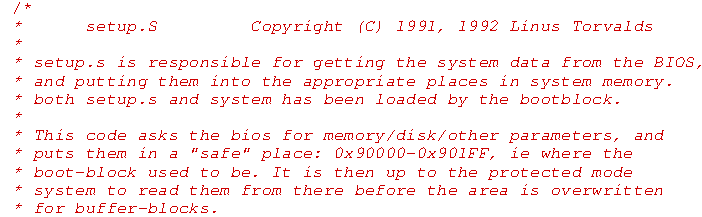
\includegraphics[width=\textwidth]{setup2} }
    \mode<article>{ 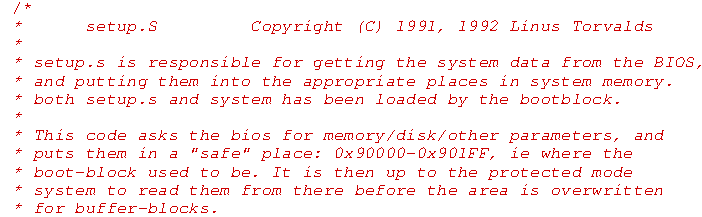
\includegraphics[width=.7\textwidth]{setup2} }
  \end{center}
  \begin{itemize}
  \item \texttt{2.6.11/arch/i386/boot/setup.S}
  \item Re-initialize all the hardware devices
  \item Sets the A20 pin (turn off \emph{wrapping around})
  \item Sets up a provisional IDT and a provisional GDT
  \item \texttt{PE=1, PG=0} in \texttt{cr0}
  \item jump to \texttt{startup\_32()}
  \end{itemize}
\end{frame}

See also:
\begin{itemize}
\item \citetitle{newbies:kernelstart}
\item \citetitle{blogspot:bootprocess}
\item \citetitle{blogspot:bootprocess2}
\end{itemize}

\begin{itemize}
\item \emph{Kernel attributes} are stored at the end of the boot block
  (1\textsuperscript{st} sector).
  (line \href{http://lxr.linux.no/linux+v2.6.11/arch/i386/boot/bootsect.S\#L90}{90} in
    \texttt{bootsect.S})
\end{itemize}  

\paragraph{The \texttt{setup()} function details:}

\begin{enumerate}
\item Builds system's physical memory map \citetitle[sec.~1.1, \emph{Memory
    Detection}]{abhishek2002memory}. See also:
  \begin{itemize}
  \item \texttt{2.4.19/arch/i386/boot/setup.S}, line
    \href{http://lxr.linux.no/linux-old+v2.4.19/arch/i386/boot/setup.S\#L289}{289-389}
  \item \texttt{2.6.11/arch/i386/boot/setup.S}, line
    \href{http://lxr.linux.no/linux+v2.6.11/arch/i386/boot/setup.S\#L302}{302-347}
  \item See also: \citetitle{wiki:e820}
  \item \url{http://www.uruk.org/orig-grub/mem64mb.html}
  \end{itemize}
\item Sets the keyboard repeat delay and rate
\item Initializes the video adapter card
\item Reinitializes the disk controller and determines the hard disk parameters
\item Checks for an IBM Micro Channel bus (MCA)
\item Checks for a PS/2 pointing device (bus mouse)
\item Checks for Advanced Power Management (APM ) BIOS support
\item If the BIOS supports the Enhanced Disk Drive Services (EDD ), builds a table in RAM
  describing the hard disks available in the system
\item If the kernel image was loaded low in RAM (at physical address \texttt{0x00010000}),
  the function moves it to physical address \texttt{0x00001000} (was used by boot loader).
  \begin{description}
  \item[Why?] This step is necessary because to be able to store the kernel image on a
    floppy disk and to reduce the booting time, the kernel image stored on disk is
    compressed, and the decompression routine needs some free space to use as a temporary
    buffer following the kernel image in RAM.  \citetitle[Sec.~A.3, \emph{Middle Ages: the
      \texttt{setup()} Function}]{bovet2005understanding}
    \begin{itemize}
    \item \texttt{BOOTSEG = 0x07C0}. This is 27K above \texttt{0x1000}. It was too small to
      hold the kernel image. After boot loader is done, \texttt{BOOTSEG (0x7C00)} is
      free. So kernel image can be stuffed here.
    \end{itemize}
  \item[Memory layout] \citetitle{blogspot:bootprocess}\,
    \begin{description}
    \item[uncompressed image:] ... Later, all the kernel is moved from \texttt{0x10000}
      (64K) to \texttt{0x1000} (4K). This move overwrites BIOS data stored in RAM, so BIOS
      calls can no longer be performed. We don't care because linux doesn't use BIOS to
      access the hardware. The first physical page is not touched because it is the
      so-called ``zero-page'', used in handling virtual memory.  At this point,
      \texttt{setup.S} enters protected mode and jumps to \texttt{0x1000}, where the kernel
      lives. All the available memory can be accessed now, and the system can begin to
      run.

      The steps just described were once the whole story of booting when the kernel was
      small enough to fit in half a megabyte of memory --- the address range between
      \texttt{0x10000} and \texttt{0x90000}. As features were added to the system, the kernel
      became larger than half a megabyte and could no longer be moved to
      \texttt{0x1000}. Thus, code at \texttt{0x1000} is no longer the Linux kernel, instead
      the “gunzip” part of the gzip program resides at that address.
      
    \item[Compressed image (zImage):] When the kernel is moved to \texttt{0x1000} (4K),
      \texttt{head.S} in the compressed directory is sitting at this address. It's in charge
      of gunzipping the kernel, this done by a function \texttt{decompress\_kernel()},
      defined in \texttt{compressed/misc.c}, which in turns calls \texttt{inflate()} which
      writes its output starting at address \texttt{0x100000} (1MB). High memory can now
      be accessed, because \texttt{setup.S} han take us to the protected mode now.  After
      decompression, \texttt{head.S} jumps to the actual beginning of the kernel. The
      relevant code is in \texttt{../kernel/head.S}. \texttt{head.S} (i.e., the code
      found at \texttt{0x100000}) can complete processor initialization and call
      \texttt{start\_ kernel()}.

      The boot steps shown above rely on the assumption that the compressed kernel can fit
      in half a megabyte of space. While this is true most of the time, a system stuffed
      with device drivers might not fit into this space. For example, kernels used in
      installation disks can easily outgrow the available space. To solve this problem
      problem bzImage kernel images were introduced.

    \item[Big Compressed Image (bzImage):] This kind of kernel image boots similarly to
      zImage, with a few changes.
    \end{description}
    When the system is loaded at \texttt{0x10000} (64K) a special helper routine is called
    which does some special BIOS calls to move the kernel to \texttt{0x100000}
    (1Mb). \texttt{setup.S} doesn't move the system back to \texttt{0x1000} (4K) but, after
    entering protected mode, jumps instead directly to address \texttt{0x100000} (1MB) where
    data has been moved by the BIOS in the previous step.  The decompresser found at 1MB
    writes the uncompressed kernel image into low memory until it is exhausted, and then
    into high memory after the compressed image.  The two pieces are then reassembled to
    the address \texttt{0x100000} (1MB). Several memory moves are needed to perform the task
    the address \texttt{0x100000} (1MB). Several memory moves are needed to perform the task
    correctly.
  \end{description}

  \begin{center}
    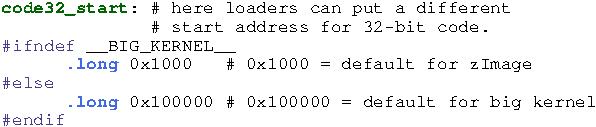
\includegraphics[width=.5\textwidth]{setup-func-1}
  \end{center}

  The default value of \texttt{code32} is \texttt{\_\_BOOT\_CS:0x1000} (\texttt{\_\_BOOT\_CS} =
  16). (Line
  \href{http://lxr.linux.no/linux+v2.6.11/arch/i386/boot/setup.S\#L855}{855-857})

  \begin{center}
    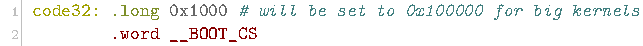
\includegraphics[width=.6\textwidth]{setup-func-2}
  \end{center}

  It will be changed to \texttt{\_\_BOOT\_CS:0x100000}.
  (Line \href{http://lxr.linux.no/linux+v2.6.11/arch/i386/boot/setup.S\#L594}{594-595})
    
  \begin{center}
    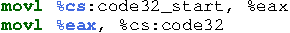
\includegraphics[width=.3\textwidth]{setup-func-3}
  \end{center}

  \texttt{\%cs:code32\_start} $\Rightarrow$ \texttt{\%cs:code32} = \texttt{0x10:0x100000} (for
  load high, i.e. \texttt{bzImage})
\item Sets the A20 pin \citetitle{wiki:a20} located on the 8042 keyboard controller (for
  switching to pmode)
\item Sets up a provisional Interrupt Descriptor Table (IDT) \citetitle{wiki:idt} and a
  provisional Global Descriptor Table (GDT) \citetitle{wiki:gdt}.
  \begin{itemize}
  \item line \href{http://lxr.linux.no/linux+v2.6.11/arch/i386/boot/setup.S\#L792}{792} in
      \texttt{setup.S}
  \item line \href{http://lxr.linux.no/linux+v2.6.11/include/asm-i386/segment.h\#L83}{83-89}
      in \texttt{include/asm-i386/segment.h}
  \end{itemize}
  The provisional GDT is created with 2 useful entries, each covering the whole 4GB
  address space \citetitle[Sec.~1.2, \emph{Provisional GDT}]{abhishek2002memory}. The code that
  loads the GDT is:    
  \begin{center}
    \includegraphics[width=.6\textwidth]{setup-func-4}
  \end{center}

  \begin{itemize}
  \item \texttt{\%ds = \%cs = SETUPSEG = 0x9020}
  \item \texttt{\$gdt} --- beginning address of the GDT table (somewhere offsetting in
    \texttt{\%ds}). Its actual value will be determined at assemble time by the assembler
    \citetitle[p24]{bartlett2009programming}
  \item \texttt{gdt\_48}: a label in \texttt{setup.S} (Line
    \href{http://lxr.linux.no/linux+v2.6.11/arch/i386/boot/setup.S\#L1006}{1006}). \texttt{gdt\_48+2}
    will be filled with the \emph{gdt base} computed above.
  \item \texttt{lgdt}: loads the value in \texttt{gdt\_48} into \texttt{GDTR}
  \item \texttt{gdt\_48 = limit,base} $\Rightarrow$ \texttt{GDTR}
    \begin{itemize}
    \item \texttt{limit = gdt\_end - gdt - 1 = 31} (16 bits)
    \item \texttt{base = \%ds $\ll$ 4 + gdt} (32 bits)
    \end{itemize}
  \end{itemize}

  \begin{center}
    \includegraphics[width=.5\textwidth]{setup-func-5}
  \end{center}

  \begin{itemize}
  \item \texttt{gdt}: the provisional GDT has 4 entries.
    \begin{itemize}
    \item The 1\textsuperscript{st} and 2\textsuperscript{nd} entries are initialized to
      0\footnote{\texttt{.fill REPEAT,SIZE,VALUE}}
      (Line \href{http://lxr.linux.no/linux+v2.6.11/arch/i386/boot/setup.S\#L983}{983}), as
      required by Intel.
      \begin{center}
        \mintinline{gas}{.fill GDT_ENTRY_BOOT_CS,8,0}
      \end{center}
    \item The 3\textsuperscript{rd} is \texttt{\_\_BOOT\_CS}
    \item The 4\textsuperscript{th} is \texttt{\_\_BOOT\_DS}
    \end{itemize}
    Calculate the linear base address of the kernel GDT (table) and load the GDT pointer
    register with its base address and limit. \citetitle[\emph{Prepare to move to protected
      mode}]{howto:init}
    \begin{figure}[h]
      \centering
      \includegraphics[width=.3\textwidth]{gdt-boot}
      \caption{Provisional GDT in RAM}
      \label{fig:gdt-boot}
    \end{figure}
    \begin{itemize}
    \item This early kernel GDT describes kernel code as 4 GB, with base address 0,
      code/readable/executable, with granularity of 4 KB.
      \begin{figure}[h]
        \centering
        \includegraphics[width=.6\textwidth]{gdt-entry-cs}
        \caption{Code segment descriptor value: \texttt{0x00CF9A000000FFFF}}
        \label{fig:cs}
      \end{figure}
    \item The kernel data segment is described as 4 GB, with base address 0,
      data/readable/writable, with granularity of 4 KB.
      \begin{figure}[h]
        \centering
        \includegraphics[width=.6\textwidth]{gdt-entry-ds}
        \caption{Data segment descriptor value: \texttt{0x00CF92000000FFFF}}
        \label{fig:ds}
      \end{figure}
    \end{itemize}
  \end{itemize}
\item Resets the floating-point unit (FPU), if any.
\item Reprograms the Programmable Interrupt Controllers (PIC) to mask all interrupts,
  except IRQ2 which is the cascading interrupt between the two PICs.
\item Switches the CPU from Real Mode to Protected Mode by setting the \texttt{PE} bit in
  the \texttt{cr0} status register. The \texttt{PG} bit in the \texttt{cr0} register is cleared,
  so paging is still disabled. (Line
  \href{http://lxr.linux.no/linux+v2.6.11/arch/i386/boot/setup.S\#L832}{832-833})

  \begin{center}
    \includegraphics[width=.4\textwidth]{setup-func-6}
  \end{center}

  \begin{itemize}
  \item \texttt{lmsw} --- Load Machine Status Word (part of
    \texttt{cr0}) \citetitle[Ch.~17]{intel86}
  \item in later kernel (e.g. 2.6.34) the switching code is like this
    (\href{http://lxr.linux.no/linux+v2.6.34/arch/x86/boot/pmjump.S\#L39}{line 39-41 in
      pmjump.S}):
      
    \begin{center}
      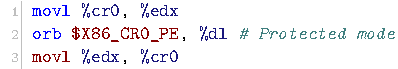
\includegraphics[width=.4\textwidth]{setup-func-7}
    \end{center}
      
    Line
    \href{http://lxr.linux.no/linux+v2.6.34/arch/x86/include/asm/processor-flags.h\#L29}{29}
    in \texttt{processor-flags.h}:
    \begin{center}
\begin{ccode}
#define X86_CR0_PE 0x00000001
\end{ccode}    
    \end{center}
  \end{itemize}
  \textbf{NOTE:} We are now in 32-bit protected mode. From now on, the address translation
  will be done by looking up the GDT table.
\item Jumps to the \texttt{startup\_32()} assembly language
  function. (Line \href{http://lxr.linux.no/linux+v2.6.11/arch/i386/boot/setup.S\#L854}{854})
  \begin{center}
    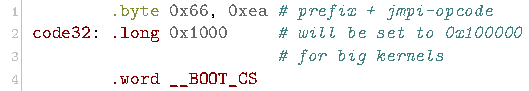
\includegraphics[width=.5\textwidth]{setup-func-8}
  \end{center}

  \begin{itemize}
  \item \mintinline{gas}{jmpi 0x100000, __BOOT_CS} (far jump)
    \begin{itemize}
    \item jump to \texttt{0x10:0x100000} (segment number: \texttt{0x10}; offset:
      \texttt{0x100000}.)
    \end{itemize}
  \item At the end of the initial assembly code in \texttt{arch/i386/boot/setup.S} a jump
    to offset \texttt{0x100000} in segment \texttt{KERNEL\_CS} is called. This is where
    the version of \mintinline{c}{startup_32()} found in
    \texttt{arch/i386/boot/compress-ed/head.S}. But the jump is a little tricky, as we
    haven't yet reloaded the \texttt{CS} register, the default size of the target offset
    still is 16 bit. However, using an operand prefix (\texttt{0x66}), the CPU will
    properly take our 48 bit far pointer [\mintinline{gas}{.byte 0x66, 0xea}]. \citetitle{blogspot:bootprocess}
  \end{itemize}
\end{enumerate}

% \begin{frame}{The real-mode kernel header}
%   The action starts in \emph{the real-mode kernel header}
%   \begin{itemize}
%   \item This region of memory is used to implement the Linux boot protocol between the
%     boot loader and the kernel
%   \item \emph{Documentation/i386/boot.txt}
%   \end{itemize}
% \end{frame}

% \begin{frame}{The real-mode kernel header}
%   \begin{block}{\emph{arch/i386/boot/bootsect.S}}
%     \begin{center}
%       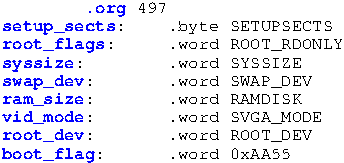
\includegraphics[width=.7\textwidth]{kernel-header}
%     \end{center}
%   \end{block}
%   \cfbox{red}{hd -n512 /boot/vmlinuz-x.x.x-x-x}
% \end{frame}

\subsubsection{\texttt{startup\_32()}}

\begin{frame}{\texttt{setup() -> startup\_32()}}%{The real mode entry point}
  \begin{block}{\texttt{startup\_32()} for compressed kernel}
    \begin{itemize}
    \item in \texttt{arch/i386/boot/compressed/head.S}
      \begin{itemize}
      \item physically at
        \begin{itemize}
        \item[]\texttt{0x00100000} --- load high, or
        \item[]\texttt{0x00001000} --- load low
        \end{itemize}
      \item does some basic register initialization
      \item \texttt{decompress\_kernel()}
      \end{itemize}
    \item the uncompressed kernel image has overwritten the compressed one starting at 1MB
    \item jump to the protected-mode kernel entry point at 1MB of RAM ($\mathtt{0x10000\ll 4}$)
      \begin{itemize}
      \item \texttt{startup\_32()} for real kernel
      \end{itemize}
    \end{itemize}
  \end{block}
\end{frame}

\paragraph{Initializing registers}
(Line \href{http://lxr.linux.no/linux+v2.6.11/arch/i386/boot/compressed/head.S\#L31}{31}
in \texttt{head.S})

\begin{center}
  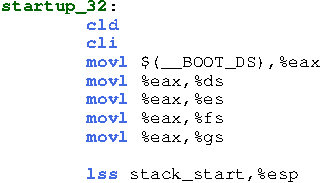
\includegraphics[width=.3\textwidth]{head-reg-init}
\end{center}

\begin{itemize}
\item \texttt{cld}: clear direction flag
\item \texttt{cli}: clear interrupt flag
\item \verb|lss stack_start, %esp|: load \texttt{\%ss} and \texttt{\%esp} pair
  (\texttt{\%ss:\%esp}) in a single instruction using the value stored in
  \texttt{stack\_start}.  (Line
  \href{http://lxr.linux.no/linux+v2.6.11/arch/i386/boot/compressed/head.S\#L40}{40} in
  \texttt{head.S})
  \begin{itemize}
  \item \texttt{lss} --- read a full pointer from memory and store it in the selected
    segment register:register pair. \citetitle[p332]{intel86}
  \end{itemize}
  % load values stored in \code{stack\_start} into \code{ss:esp}
\item \texttt{stack\_start} (Line
  \href{http://lxr.linux.no/linux+v2.6.11/arch/i386/boot/compressed/misc.c\#L296}{296-303}
  in \texttt{misc.c})

  \begin{center}
    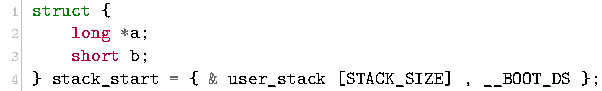
\includegraphics[width=.6\textwidth]{stack-start}
  \end{center}

\item \texttt{STACK\_SIZE} = 4096
\item \texttt{\_\_BOOT\_DS} = 24 (segment selector) $\Rightarrow$ \texttt{\%ss}
  \begin{itemize}
  \item the 4\textsuperscript{th} (2\textsuperscript{nd} non-zero) entry in provisional
    GDT \citetitle[Sec.~1.2, \emph{Provisional GDT}]{abhishek2002memory}. Each entry is
    8 bytes.
  \end{itemize}
\item \texttt{\&user\_stack[4096]} $\Rightarrow$ \texttt{\%esp}
\end{itemize}

\paragraph{Clear BSS}

(Line
\href{http://lxr.linux.no/linux+v2.6.11/arch/i386/boot/compressed/head.S\#L55}{55} in
\texttt{head.S})

\begin{center}
  \includegraphics[width=.2\textwidth]{head-clr-bss}
\end{center}
  
\begin{itemize}
\item \href{http://www.cs.ubbcluj.ro/\char`~dadi/ac/doc/ng1d5fc.html}{\texttt{stosb}} copies the
  value in \texttt{AL} into the location pointed to by \texttt{ES:DI}. \texttt{DI} is then
  incremented (if the direction flag is cleared) or decremented (if the direction flag is
  set), in preparation for storing \texttt{AL} in the next location.
\item \texttt{rep} --- repeat
\item For \texttt{ecx} repetitions, stores the contents of \texttt{eax} into where \texttt{edi}
  points to, incrementing or decrementing \texttt{edi} (depending on the direction flag) by
  4 bytes each time. Normally, this is used for a memset-type operation.

  Usually, that instruction is simply written ``\mintinline{gas}{rep stosd}''. Experienced assembly
  coders know all the details mentioned above just by seeing that. \good{}%:-)

  ETA for completeness (thanks PhiS): Each iteration, \texttt{ecx} is decremented by 1, and
  the loop stops when it reaches zero. For \texttt{stos}, the only thing you will observe is
  that \texttt{ecx} is cleared at the end. \citetitle{stack:stos}
\end{itemize}

\begin{frame}{\texttt{startup\_32()} for real kernel}
  \begin{block}{\texttt{startup\_32()} in \texttt{arch/i386/kernel/head.S}}
    \begin{itemize}
    \item Zeroes the kernel BSS for protected mode
    \item sets up the final GDT
    \item builds provisional kernel page tables so that paging can be turned on
    \item enables paging (\texttt{cr3->PGDir; PG=1} in \texttt{cr0})
    \item initializes a stack
    \item \texttt{setup\_idt()} --- creates the final interrupt descriptor table
    \item \texttt{gdtr->GDT; idtr->IDT}
    \item \texttt{start\_kernel()}
    \end{itemize}
  \end{block}
\end{frame}

\paragraph{Sets up the final GDT}

(line \href{http://lxr.linux.no/linux+v2.6.11/arch/i386/kernel/head.S\#L63}{63},
\href{http://lxr.linux.no/linux+v2.6.11/arch/i386/kernel/head.S\#L303}{303},
\href{http://lxr.linux.no/linux+v2.6.11/arch/i386/kernel/head.S\#L448}{448-450},
\href{http://lxr.linux.no/linux+v2.6.11/arch/i386/kernel/head.S\#L459}{459-463},
\href{http://lxr.linux.no/linux+v2.6.11/arch/i386/kernel/head.S\#L470}{470-EOF} in \texttt{head.S})

\begin{center}
  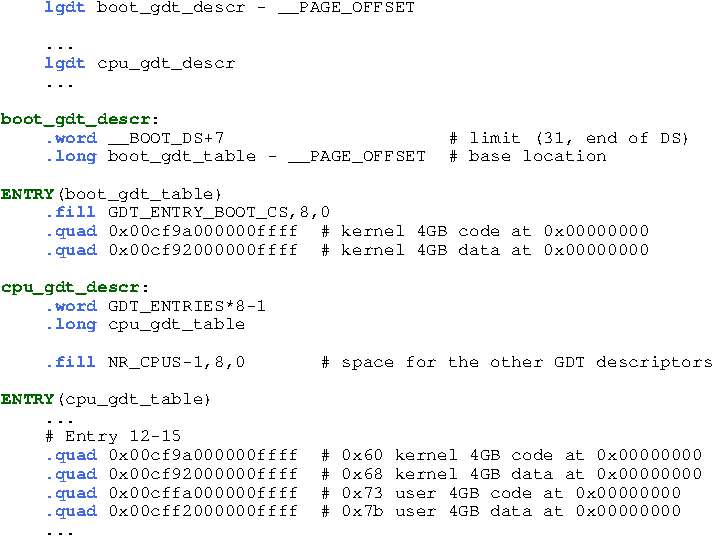
\includegraphics[width=.7\textwidth]{head-gdt-setup}
\end{center}
  
\begin{itemize}
\item \texttt{.fill REPEAT, SIZE, VALUE}
  \begin{itemize}
  \item \mintinline{gas}{.fill 2,8,0} --- fills the 1\textsuperscript{st} and
    2\textsuperscript{nd} entry with \texttt{0}
  \end{itemize}
\item \texttt{.quad} 8-byte datas (the 3\textsuperscript{rd} and 4\textsuperscript{th}
  entry)
\item The addresses of \texttt{boot\_gdt\_table} and \texttt{cpu\_gdt\_table} will be assigned
  by assembler at compile time.
\end{itemize}

\paragraph{Zeroes the kernel BSS}
(line 74-79 in \texttt{arch/i386/kernel/head.S})

\begin{center}
  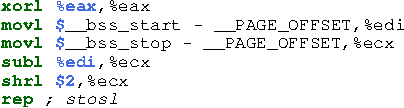
\includegraphics[width=.4\textwidth]{head-kernel-bss-init}
\end{center}
  
\begin{itemize}
\item \mintinline{gas}{subl %edi, %ecx} --- get BSS size, put into \texttt{\%ecx}
  \item \mintinline{gas}{shrl $2, %ecx} --- %$
      $\mathtt{\frac{\%ecx}{4}}$, get number of 4-byte chunks (repeat times)
\item
  \href{http://pdos.csail.mit.edu/6.828/2004/readings/i386/STOS.htm}{\texttt{stosl}/\texttt{stosd}}
  --- Store \texttt{EAX} in dword \texttt{ES:EDI}, update \texttt{EDI}
\end{itemize}

\paragraph{Initialize page tables}
\citetitle[Sec.~2.5.5, \emph{Kernel Page Tables}]{bovet2005understanding}

In the first phase, the kernel creates a limited address space including the kernel's code
and data segments, the initial Page Tables, and 128 KB for some dynamic data
structures. This minimal address space is just large enough to install the kernel in RAM
and to initialize its core data structures.

The provisional Page Global Directory is contained in the \texttt{swapper\_pg\_dir}
variable. \texttt{swapper\_pg\_dir} is at the beginning of BSS (uninitialized data area)
because BSS is no longer used after system start up.

The provisional Page Tables are stored starting from \texttt{pg0}, right after the end of
the kernel's uninitialized data segments (\texttt{\_end}).

For the sake of simplicity, let's assume that the kernel's segments, the provisional Page
Tables, and the 128 KB memory area fit in the first 8 MB of RAM. In order to map 8 MB of
RAM, two Page Tables are required.

The objective of this first phase of paging is to allow these 8 MB of RAM to be easily
addressed both in real mode and protected mode.

\begin{center}
  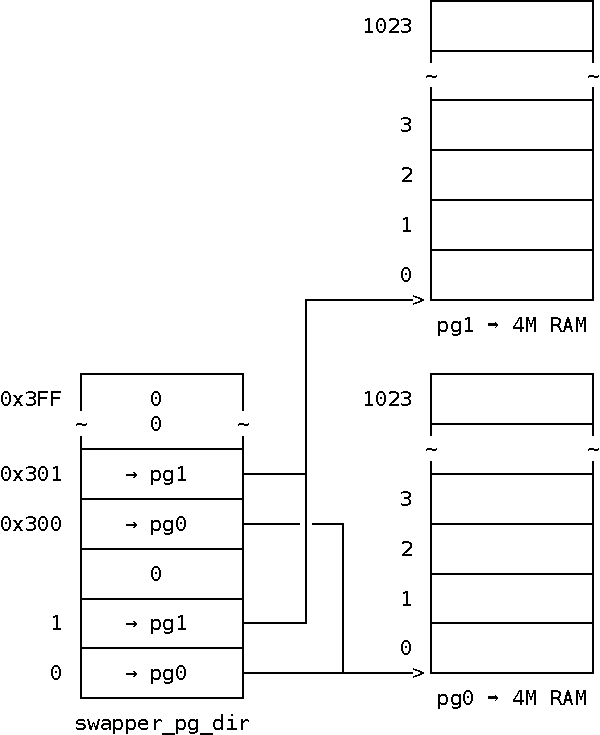
\includegraphics[width=.4\textwidth]{kernel-page-table-boot}
\end{center}

Therefore, the kernel must create a mapping from both the linear addresses
\texttt{0x00000000} through \texttt{0x007fffff} (8M) and the linear addresses
\texttt{0xc0000000} through \texttt{0xc07fffff} (8M) into the physical addresses
\texttt{0x00000000} through \texttt{0x007fffff}. In other words, the kernel during its
first phase of initialization can address the first 8 MB of RAM by either linear addresses
identical to the physical ones or 8 MB worth of linear addresses, starting from
\texttt{0xc0000000}.

\subparagraph{Why?}

From \citetitle[Sec.~1.3.2, \emph{Provisional Kernel Page Tables}]{abhishek2002memory}:
  
\begin{itemize}
\item All pointers in the compiled kernel refer to addresses $> PAGE\_OFFSET$. That is,
  the kernel is linked under the assumption that its base address will be
  \texttt{start\_text} (I think; I don't have the code on hand at the moment), which is
  defined to be $PAGE\_OFFSET+(some\ small\ constant,\ call\ it\ C)$.
\item All the kernel bootstrap code (mostly real mode code) is linked assuming that its
  base address is $0+C$.
\end{itemize}

\texttt{head.S} is part of the bootstrap code. It's running in protected mode with paging
turned off, so all addresses are physical. In particular, the instruction pointer is
fetching instructions based on physical address. The instruction that turns on paging
(\mintinline{gas}{movl %eax, %cr0}) is located, say, at some physical address \texttt{A}.

As soon as we set the paging bit in \texttt{cr0}, paging is enabled, and starting at the
very next instruction, all addressing, including instruction fetches, pass through the
address translation mechanism (page tables). IOW, all address are henceforth virtual. That
means that

\begin{enumerate}
\item We must have valid page tables, and
\item Those tables must properly map the instruction pointer to the next instruction to be
  executed.
\end{enumerate}

That next instruction is physically located at address \texttt{A+4} (the address immediately
after the "\mintinline{gas}{movl %eax, %cr0}" instruction), but from the point of view of all the
kernel code --- which has been linked at \texttt{PAGE\_OFFSET} --- that instruction is
located at virtual address \texttt{PAGE\_OFFSET+(A+4)}. Turning on paging, however, does not
magically change the value of EIP \footnote{The value of EIP is still physically
  \texttt{A+4}, not \texttt{PAGE\_OFFSET+(A+4)} yet. But since paging is just enabled, CPU
  could pass \texttt{A+4} through address translation.}.  The CPU fetches the next
instruction from ***virtual*** address \texttt{A+4}; that instruction is the beginning of a
short sequence that effectively relocates the instruction pointer to point to the code at
\texttt{PAGE\_OFFSET + A + (something)}.

But since the CPU is, for those few instructions, fetching instructions based on physical
addresses ***but having those instructions pass through address translation***, we must
ensure that both the physical addresses and the virtual addresses are :

\begin{enumerate}
\item Valid virtual addresses, and
\item Point to the same code.
\end{enumerate}

That means that at the very least, the initial page tables must

\begin{enumerate}
\item map virtual address \texttt{PAGE\_OFFSET+(A+4)} to physical address \texttt{(A+4)}, and
  must
\item map virtual address \texttt{A+4} to physical address \texttt{A+4}.
\end{enumerate}

This dual mapping for the first 8MB of physical RAM is exactly what the initial page
tables accomplish. The 8MB initally mapped is more or less arbitrary. It's certain that no
bootable kernel will be greater than 8MB in size. The identity mapping is discarded when
the MM system gets initialized.
  
\begin{center}
  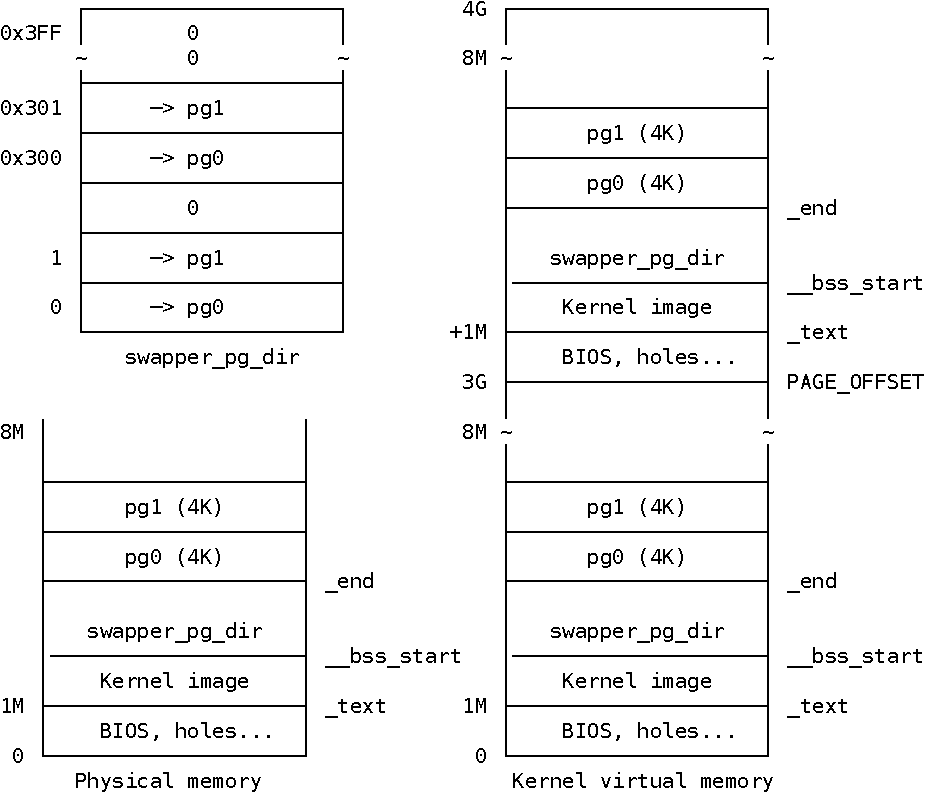
\includegraphics[width=.5\textwidth]{kernel-page-table}
\end{center}

Line \href{http://lxr.linux.no/linux+v2.6.11/arch/i386/kernel/head.S\#L91}{91-111} in
\texttt{head.S}

\begin{center}
  \includegraphics[width=.8\textwidth]{head-kernel-pgt-init}
\end{center}
  
\begin{center}
  \includegraphics[width=.5\textwidth]{i386pte}
\end{center}

\begin{itemize}
  % \item The identity mapping is discarded when the MM system gets initialized.
\item \mintinline{c}|page_pde_offset = (__PAGE_OFFSET >> 20); /* 0xC00, the 3K point. */|
    
  The \texttt{PGDir} is one page (4K) in size. It's divided into two parts:
  \begin{enumerate}
  \item first 3K (768 entries) for user mode
  \item last 1K (256 entries) for kernel mode
  \end{enumerate}
\item \texttt{\$(pg0 - \_\_PAGE\_OFFSET)} yields the physical address of \texttt{pg0}
  since here it is a linear address. Same case for \texttt{\$(swapper\_pg\_dir -
    \_\_PAGE\_OFFSET)}.
  \begin{itemize}
  \item \texttt{swapper\_pg\_dir} starts at the beginning of BSS
  \item \texttt{pg0} starts at \texttt{\_end}
  \end{itemize}
\item Registers:
  \begin{description}
  \item[\texttt{\%edi}] address of each page table entry, i.e. \texttt{pg0[0]..pg0[1023]},
    \texttt{pg1[0]..pg1[1023]}.
  \item[\texttt{\%edx}] address of \texttt{swapper\_pg\_dir[0]}, and then to
    \texttt{swapper\_pg\_dir[1]}.
  \item[\texttt{\%ecx}] has two uses
    \begin{enumerate}
    \item contents of \texttt{swapper\_pg\_dir[0]}, \texttt{swapper\_pg\_dir[1]},
      \texttt{swapper\_pg\_dir[768]},\\ \texttt{swapper\_pg\_dir[769]}.
    \item loop counter (1024 -> 0)
    \end{enumerate}
  \item[\texttt{\%eax}] \texttt{7, 4k+7, 8k+7 ... 8M-4k+7} for 2k page table entries in
    \texttt{pg0} and \texttt{pg1} respectively.
  \item[\texttt{\%ebp}] \texttt{= 128k + 7 + \&pg0[1023]} in the first round of loop. Its
    value cannot be determined at coding time, because the address of \texttt{pg0} is
    not known until compile/link time.
  \end{description}
\item \texttt{stosl}: stores the contents of EAX at the address pointed by \texttt{EDI},
  and increments \texttt{EDI}. Equivalent to:
  \begin{center}
  \begin{gascode}
movl %eax, (%edi)
addl $4, %edi
\end{gascode}
  \end{center}
\item \texttt{cmpl, jb}: if \texttt{\%eax} < \texttt{\%ebp}, jump to 10;
  \begin{itemize}
  \item \texttt{jb}: jump on below/less than, unsigned \citetitle[Sec.~8, \emph{Program
      flow}]{wiki:x86asm}
  \item At the end of the 1\textsuperscript{st} round of loop, the value of \texttt{\%eax}
    is \texttt{4M-4k+7}, while the value of \texttt{\%ebp} depends on the address of
    \texttt{pg0}.
    
    If the kernel image is small enough (e.g. a \texttt{zImage}), \texttt{pg0} could be
    low enough to let the 128KB covered without a \texttt{pg1}.
  \end{itemize}
\item \texttt{INIT\_MAP\_BEYOND\_END}: 128KB, used as a bitmap covering all pages. For
  1M pages (4GB RAM), we need 1M bits (128K
  bytes)\footnote{dead link: \url{http://kerneldiy.com/blog/?p=201}}
\end{itemize}

\href{http://www.eefocus.com/article/09-04/71517s.html}{Equivalent pseudo C code}\footnote{\url{http://www.eefocus.com/article/09-04/71517s.html}}:

\begin{center}
  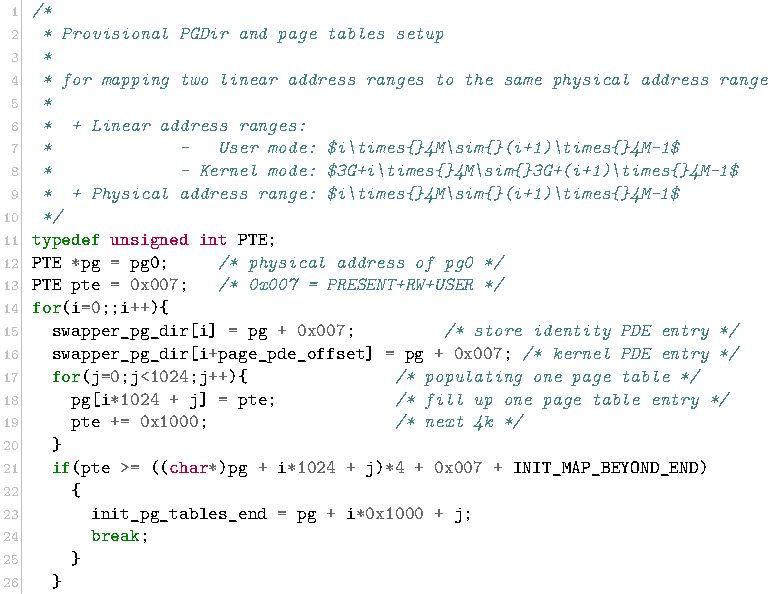
\includegraphics[width=.7\textwidth]{provisional-pgdir1}
\end{center}

\paragraph{Enable paging}

\citetitle[Sec.~6.1]{howto:i386bootcode} (Line
\href{http://lxr.linux.no/linux+v2.6.11/arch/i386/kernel/head.S\#L186}{186-194} in
\texttt{head.S})

\begin{center}
  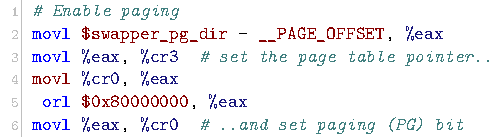
\includegraphics[width=.6\textwidth]{head6}
\end{center}
    
% \begin{frame}{start\_of\_setup}
%   \begin{itemize}
%   \item sets up a stack
%   \item zeroes the bss segment
%   \item jumps to \code{main()} in \emph{arch/x86/boot/main.c}
%   \end{itemize}
% \end{frame}

% \begin{frame}{main()}
%   \code{main()} does some house keeping like detecting memory layout, setting a video mode,
%   etc. It then calls \code{go\_to\_protected\_mode()} in \emph{arch/x86/boot/pm.c}
% \end{frame}

% \begin{frame}{go\_to\_protected\_mode()}
%   \begin{itemize}
%   \item \code{enable\_a20()} --- addressing more than 1MB in real mode
%   \item \code{setup\_idt()}
%     \begin{itemize}
%     \item in real mode the \emph{interrupt vector table} is at address 0
%     \item in protected mode, let IDTR take care of it.
%     \end{itemize}
%   \item \code{setup\_gdt()} --- put GDT's address into GDTR.
%     \begin{itemize}
%     \item GDT is used for address translation (logical $\rightarrow$ linear) in protected mode
%     \end{itemize}
%   \item \code{protected\_mode\_jump()} in \emph{arch/x86/boot/pmjump.S}
%     \begin{itemize}
%     \item setting the PE (Protected Enabled) bit in the CR0 CPU register
%     \item jumping to the 32-bit kernel entry point (\code{startup\_32()} for compressed kernel)
%     \end{itemize}
%   \end{itemize}
% \end{frame}

\subsubsection{\texttt{start\_kernel()}}

\begin{frame}
  \begin{block}{\texttt{start\_kernel()} --- a long list of calls to initialize various
      kernel subsystems and data structures}
    \begin{itemize}
    \item \texttt{sched\_init()} --- scheduler
    \item \texttt{build\_all\_zonelists()} --- memory zones
    \item \texttt{page\_alloc\_init(), mem\_init()} --- buddy system
    \item \texttt{trap\_init(), init\_IRQ()} --- IDT
    \item \texttt{time\_init()} --- time keeping
    \item \texttt{kmem\_cache\_init()} --- slab allocator
    \item \texttt{calibrate\_delay()} --- CPU clock
    \item \texttt{kernel\_thread()} --- The kernel thread for process 1
    \item login prompt
    \end{itemize}
  \end{block}
\end{frame}

% \begin{frame}{\code{rest\_init()}}
%   \code{rest\_init()} in \emph{init/main.c}
%   \begin{itemize}
%   \item \code{kernel\_thread()}
%     \begin{itemize}
%     \item \code{kernel\_thread()} $\rightarrow$ \code{kernel\_init()} $\rightarrow$ \code{init\_post()}
%       \begin{itemize}
%       \item \code{kernel\_init()} is responsible for initializing the remaining CPUs in the system
%       \item \code{init\_post()} tries to execute a user-mode process --- init starts running as
%         PID 1.
%       \end{itemize}
%     \item \code{schedule()}
%     \item \code{cpu\_idle()}
%     \end{itemize}
%   \end{itemize}
% \end{frame}

\begin{frame}{The Kernel Boot Process}
  \begin{center}
    \mode<beamer>{ 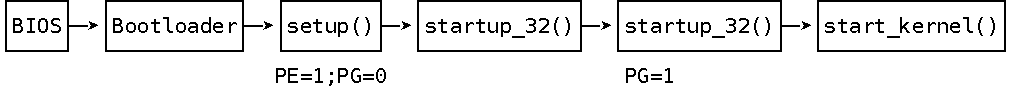
\includegraphics[width=\textwidth]{bootprocess} }
    \mode<article>{ 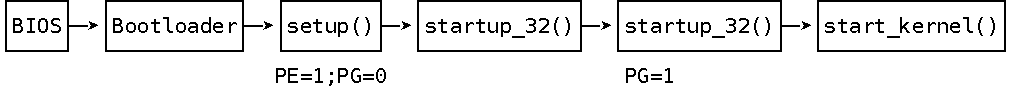
\includegraphics[width=.7\textwidth]{bootprocess} }
  \end{center}
\end{frame}

\begin{frame}{The Kernel Boot Process}
  \begin{center}
    \mode<beamer>{ 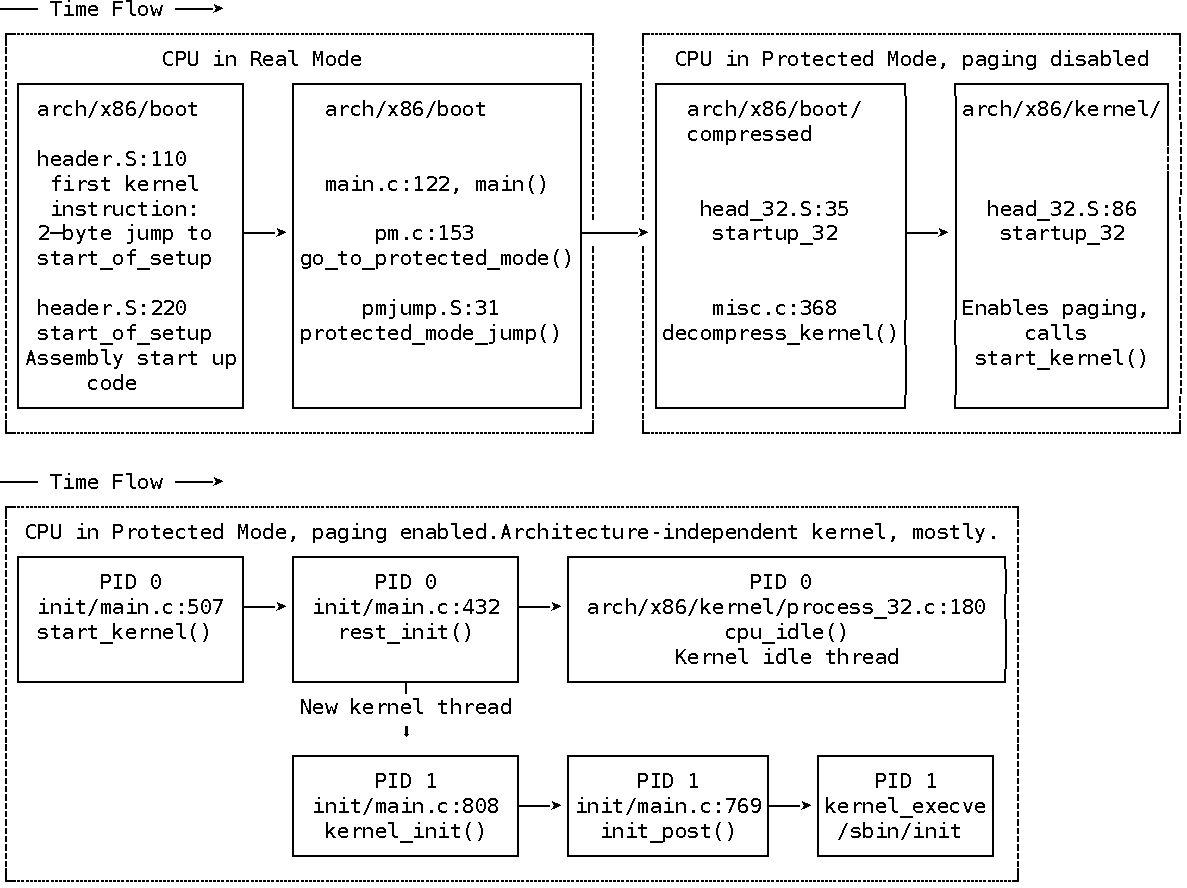
\includegraphics[width=\textwidth]{kernelInit} }
    \mode<article>{ 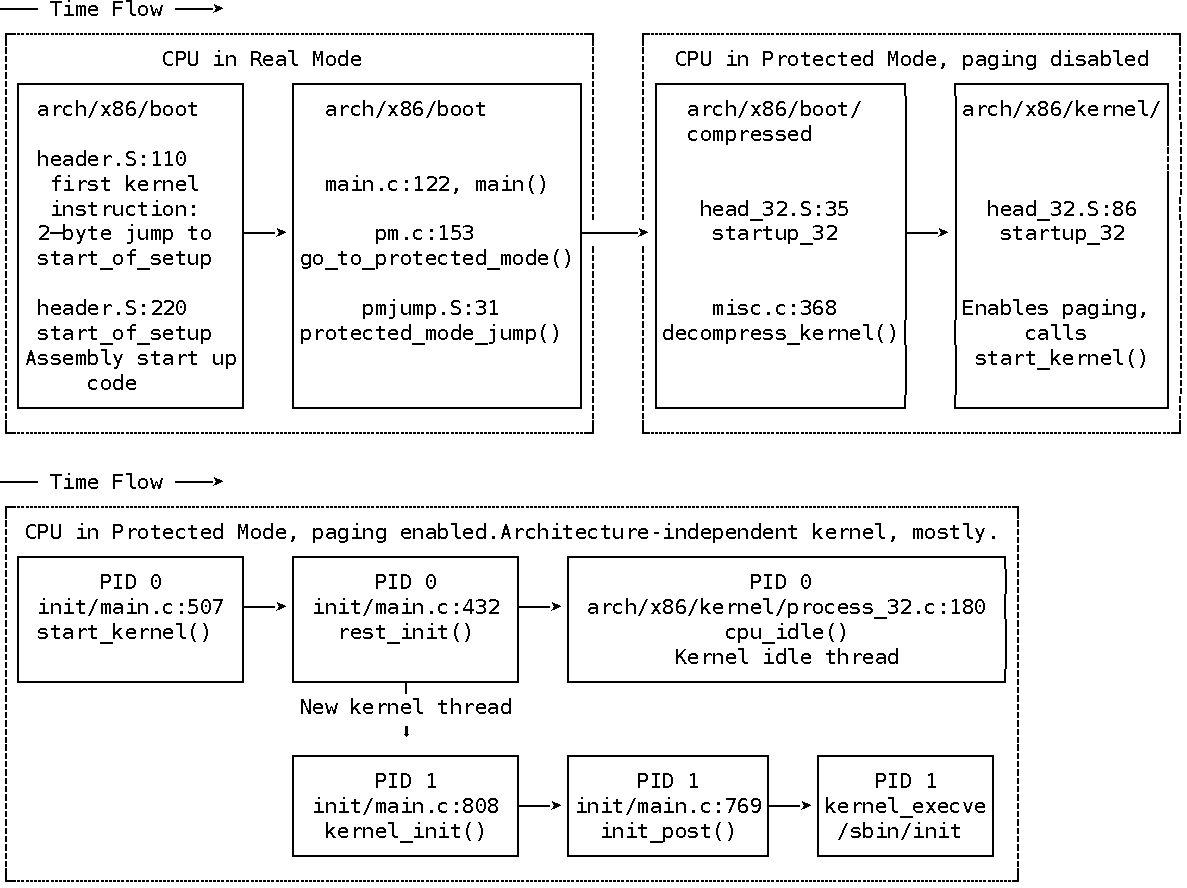
\includegraphics[width=.8\textwidth]{kernelInit} }
  \end{center}
\end{frame}

\begin{itemize}
\item This picture is not fully compatible with 2.6.11.
\end{itemize}

% \begin{frame}{The Kernel Boot Process (II)}
%   \begin{center}
%     \mode<beamer>{
%       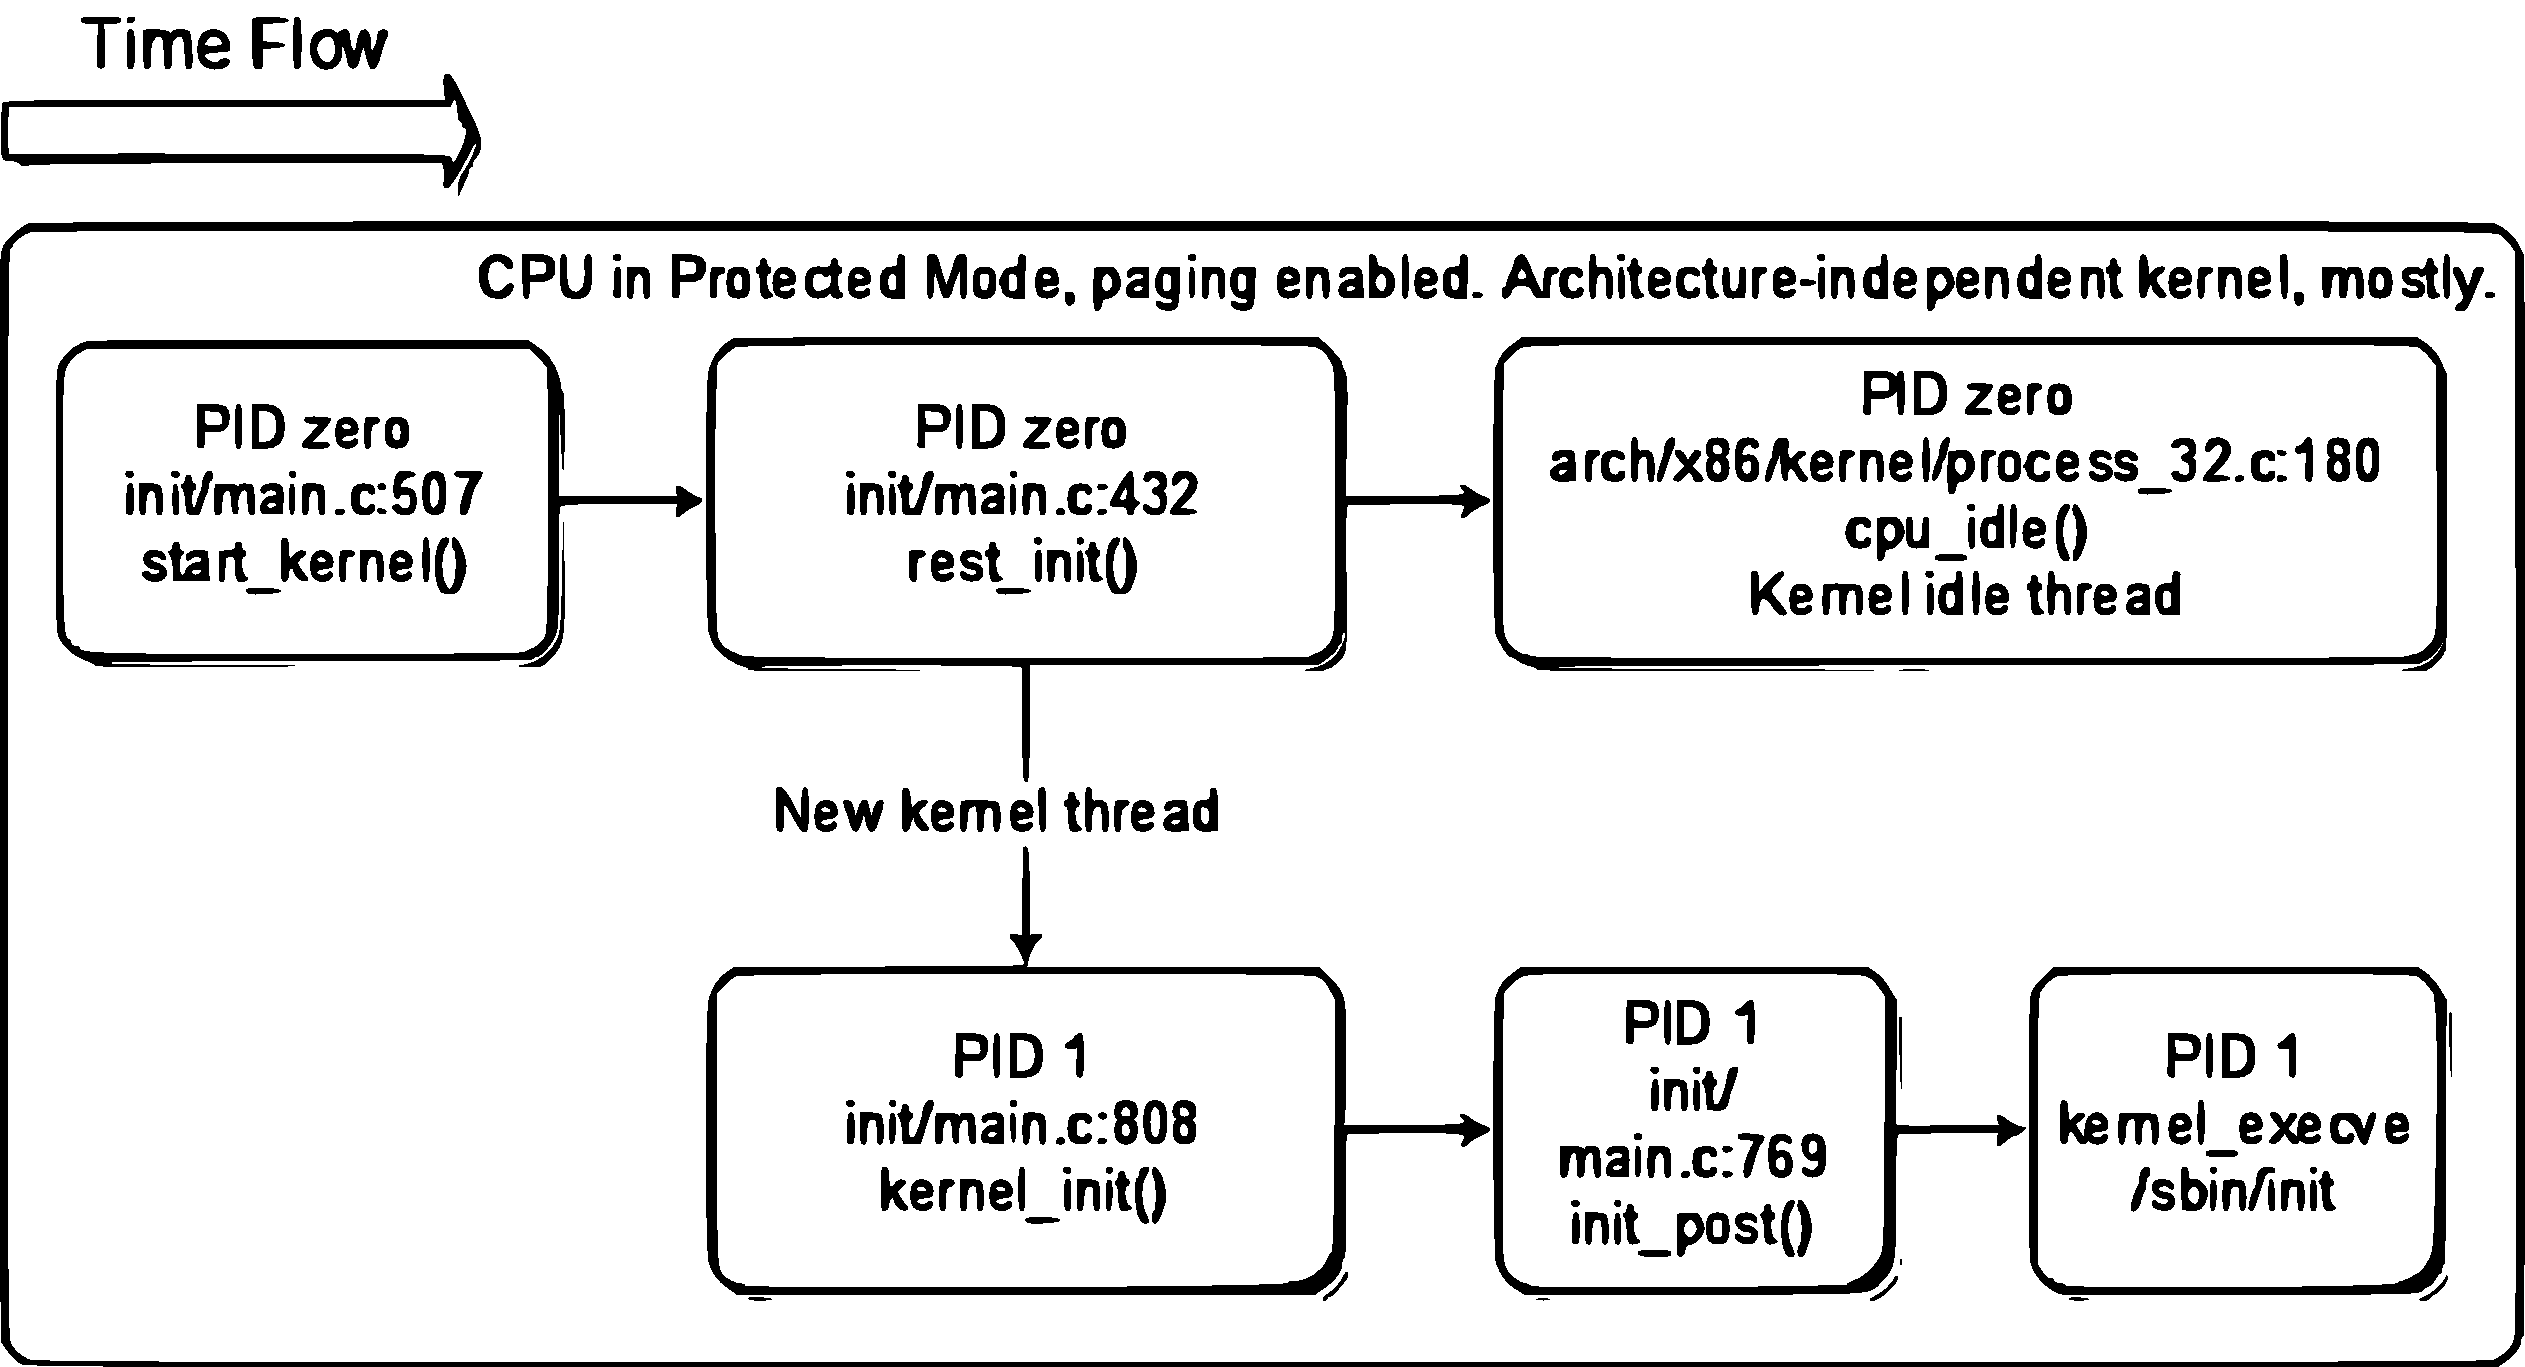
\includegraphics[width=\textwidth]{kernelInitPartTwo}
%     }
%     \mode<article>{
%       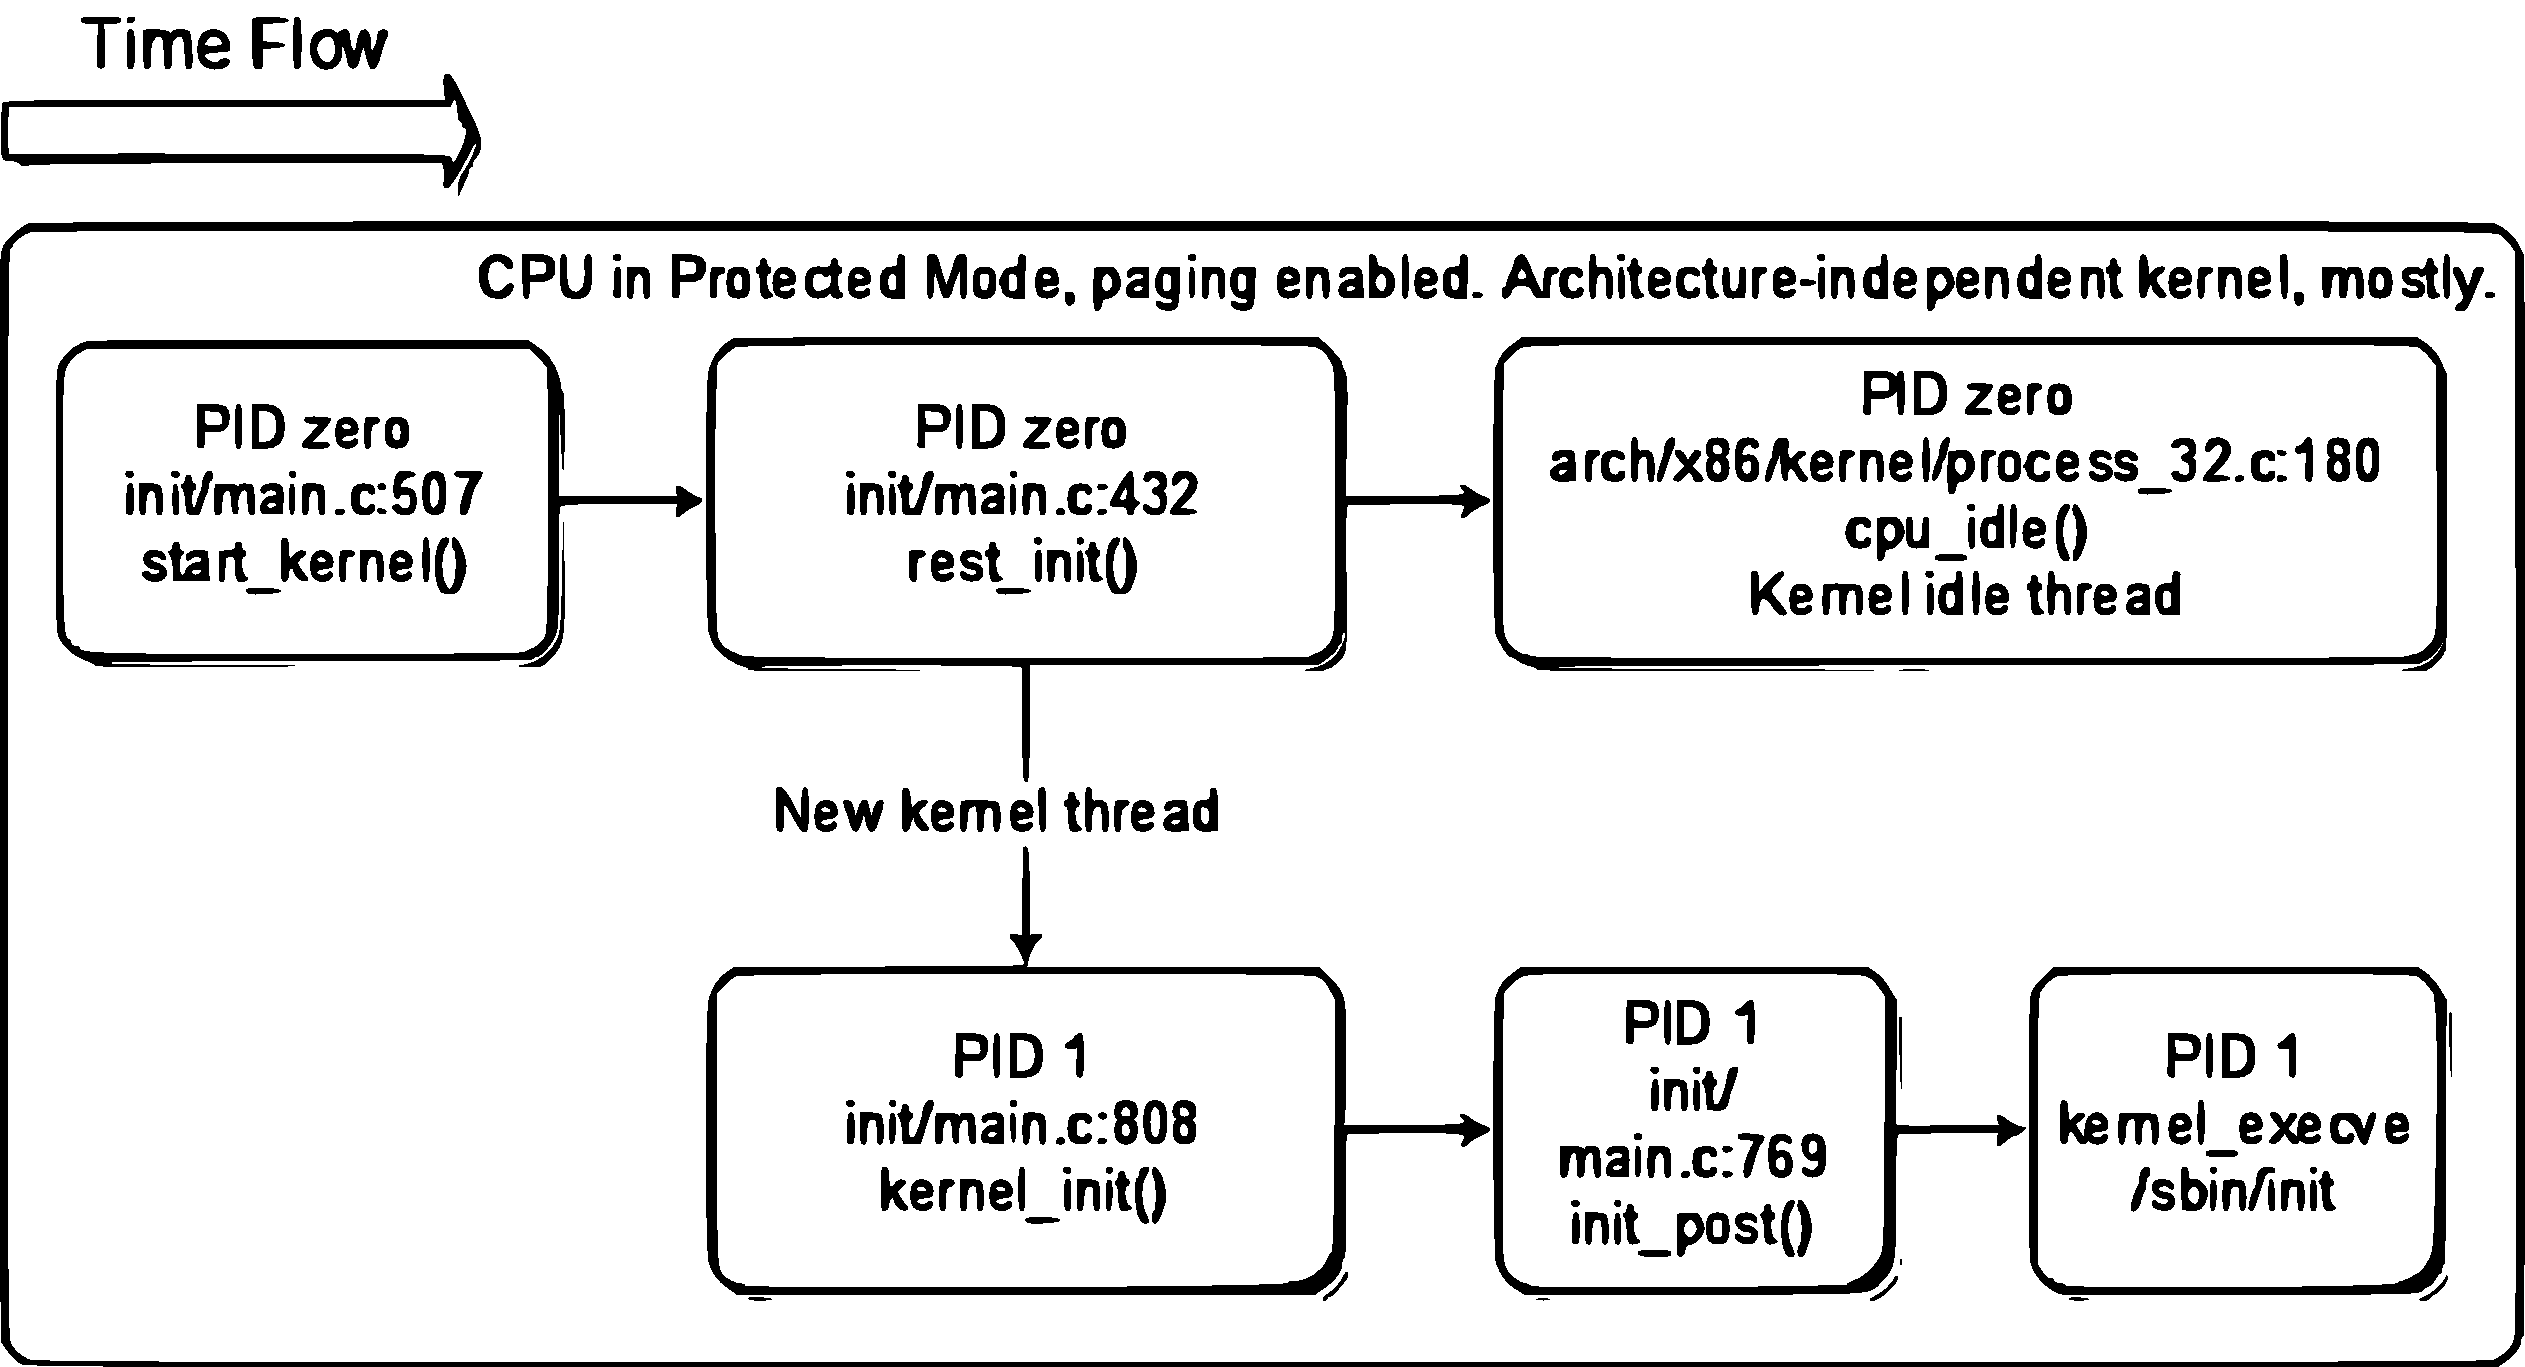
\includegraphics[width=.8\textwidth]{kernelInitPartTwo}
%     }
%   \end{center}
% \end{frame}

% \begin{itemize}
% \item This picture is not fully compatible with 2.6.11.
% \end{itemize}

\mode<all>
%%% Local Variables:
%%% mode: latex
%%% TeX-master: "kernel-b"
%%% End:
